%==========================================={ PACKAGES }============================================

\documentclass[11pt]{article}
% Article type and font.
\usepackage[margin=1in,bottom=1in,top=1in]{geometry}
% Formatting of pages in doc.
\usepackage{setspace}
% Custom control for line spacing in doc.
\usepackage{fancyhdr}
% Fancy Header Pkg.
\usepackage{amsmath}
% American Mathematical Society Math Pkg.
\usepackage{amssymb}
% American Mathematical Society Symbols Pkg.
\usepackage{fdsymbol}
% Many addtnl. mathematical operators.
\usepackage{marvosym}
% Many addtnl. useful symbols, such as for footnotes
\usepackage[dvipsnames]{xcolor}
\definecolor{Lred}{RGB}{255, 102, 102}
\definecolor{bloodorange}{RGB}{255, 83, 0}
\definecolor{Lbloodorange}{RGB}{255, 152, 102}
\definecolor{Lorange}{RGB}{255, 201, 102}
\definecolor{shininggold}{RGB}{255, 210, 0}
\definecolor{Lshininggold}{RGB}{255, 228, 102}
\definecolor{Lyellow}{RGB}{255, 255, 179}
\definecolor{leafgreen}{RGB}{128, 192, 0}
\definecolor{Lleafgreen}{RGB}{179, 217, 102}
\definecolor{hulkgreen}{RGB}{0, 128, 0}
\definecolor{Lhulkgreen}{RGB}{102, 179, 102}
\definecolor{oceanblue}{RGB}{0, 64, 128}
\definecolor{Loceanblue}{RGB}{102, 140, 179}
\definecolor{Lblue}{RGB}{102, 102, 255}
\definecolor{darkblue}{RGB}{38, 0, 193}
\definecolor{Ldarkblue}{RGB}{125, 102, 218}
\definecolor{indigo}{RGB}{75, 0, 130}
\definecolor{Lindigo}{RGB}{147, 102, 180}
\definecolor{codeblack}{RGB}{40, 36, 44}
\definecolor{codeborder}{RGB}{119,136,153}
\definecolor{macosred}{RGB}{255, 92, 84}
\definecolor{macosyellow}{RGB}{252,188,44}
\definecolor{macosgreen}{RGB}{36, 204, 67}
\definecolor{macosgrey}{RGB}{72, 68, 68}
\definecolor{macosblack}{RGB}{28, 28, 28}
\definecolor{apple}{RGB}{67, 199, 51}
\definecolor{electricviolet}{RGB}{106, 65, 246}
\definecolor{blueone}{RGB}{64, 102, 255}
\definecolor{bluetwo}{RGB}{112, 140, 255}
\definecolor{bluethree}{RGB}{160, 179, 255}
\definecolor{bluefour}{RGB}{207, 217, 255}
\definecolor{ubuntupurple}{RGB}{48, 10, 36}
\definecolor{ubuntugreen}{RGB}{38, 162, 105}
\definecolor{ubuntublue}{RGB}{19, 72, 139}
% more colors & some custom ones (L = light)
\usepackage{tikz}
% Manually draw math pictures using code
\usepackage{multicol}
% Split page into multiple columns
\usetikzlibrary{positioning}
% Useful for manually-creating graphs (e.g. lattices).
\usepackage{graphicx}
\graphicspath{ {./images/} }
% Upload images directly into doc, size them, etc.
% Uploaded images are pulled from ./images/ folder in sidebar.
\usepackage[font=small,labelfont=bf]{caption}
% Create custom captions for images, graphs, etc.
\usepackage{multirow}
\setlength{\columnseprule}{1pt}
\setlength{\columnsep}{20pt}
\def\columnseprulecolor{\color{black}}
% For tables
\usepackage{colortbl}
% For coloring cells of tables
\usepackage{arydshln}
% For dashed lines surrounding cells in tables
\usepackage[]{mdframed}
% Creates box around text: useful for code/solutions.
\usepackage{hyperref}
\hypersetup{hidelinks}
% Hyperlinks; second one makes their clickable boxes invisible
\usepackage{booktabs}
% For style lines dividing matrix elements inside.
\usepackage{textcomp}
% For straight, single quotes.
\usepackage{yfonts}
% adds fonts like gothic
% 11-color rainbow palette
\usepackage{longfbox}
\makeatletter
\newdimen\@tempdimd
\makeatother
\usepackage[many]{tcolorbox}
% for rounded boxes around text
% highlighting text (colorful)
\tcbuselibrary{skins, xparse, listings}
% for something to do with the realisitc command shell
\usepackage{pgfornament}
% for decorative symbols and such
\usepackage{array}
% need this for something table-related
\usepackage{fontspec}
% for toggling between fonts & using custom fonts (must use XeLaTeX/LuaLaTeX)
\usepackage{moresize}
% adds \HUGE and \TINY 
\usepackage{emoji}
% emojis! (must use LuaLaTeX)

%========================================{ CUSTOM COMMANDS }======================================== 

\newcommand{\Mod}[1]{\ (\mathrm{mod}\ #1)}
% Modular Arithmetic spacing + parenthesis
\NewDocumentCommand{\Customarrow}{}{\hspace{0.2cm}\rightarrow\hspace{0.2cm}}
% Large custom "implies" arrow
\NewDocumentCommand{\customarrow}{}{\hspace{0.1cm}\rightarrow\hspace{0.1cm}}
% Small custom "implies" arrow
\NewDocumentCommand{\newproblem}{mm}
{\begin{center}
    \section*{\underline{Problem #1:{}{#2}}}
\end{center}}
% New Problem: formatting, bolding, spacing, etc.
\NewDocumentCommand{\problempart}{mm}{\noindent\textbf{(#1){ } #2}}
% Part x of Problem y

\def\barroman#1{\sbox0{#1}\dimen0=\dimexpr\wd0+1pt\relax
  \makebox[\dimen0]{\rlap{\vrule width\dimen0 height 0.09ex depth 0.06ex}%
    \rlap{\vrule width\dimen0 height\dimexpr\ht0+0.06ex\relax 
            depth\dimexpr-\ht0+0.09ex\relax}%
    \kern.5pt#1\kern.5pt}}
% Roman Numerals: \barroman{letter(s)}

\newtcolorbox{redbox}[1]{colback=red!5!white,
colframe=red,fonttitle=\bfseries,
title={#1}}
% red text box

\newtcolorbox{bloodorangebox}[1]{colback=bloodorange!5!white,
colframe=bloodorange,fonttitle=\bfseries,
title={#1}}
% bloodorange text box

\newtcolorbox{orangebox}[1]{colback=orange!5!white,
colframe=orange,fonttitle=\bfseries,
title={#1}}
% orange text box

\newtcolorbox{shininggoldbox}[1]{colback=shininggold!5!white,
colframe=shininggold,fonttitle=\bfseries,
title={#1}}
% shininggold text box

\newtcolorbox{yellowbox}[1]{colback=yellow!5!white,
colframe=yellow,fonttitle=\bfseries,
title={#1}}
% yellow text box

\newtcolorbox{leafgreenbox}[1]{colback=leafgreen!5!white,
colframe=leafgreen,fonttitle=\bfseries,
title={#1}}
% leafgreen text box

\newtcolorbox{hulkgreenbox}[1]{colback=hulkgreen!5!white,
colframe=hulkgreen,fonttitle=\bfseries,
title={#1}}
% hulkgreen text box

\newtcolorbox{oceanbluebox}[1]{colback=oceanblue!5!white,
colframe=oceanblue,fonttitle=\bfseries,
title={#1}}
% oceanblue text box

\newtcolorbox{bluebox}[1]{colback=blue!5!white,
colframe=blue,fonttitle=\bfseries,
title={#1}}
% blue text box

\newtcolorbox{darkbluebox}[1]{colback=darkblue!5!white,
colframe=darkblue,fonttitle=\bfseries,
title={#1}}
% darkblue text box

\newtcolorbox{indigobox}[1]{colback=indigo!5!white,
colframe=indigo,fonttitle=\bfseries,
title={#1}}
% indigo text box

\newtcolorbox{blackbox}[1]{colback=black!5!white,
colframe=black,fonttitle=\bfseries,
title={#1}}
% black text box

\newcommand\codebox[1]{
    \noindent\hspace{-0.25em}\begin{tcolorbox}[on line, hbox, colback = codeblack, colframe = codeborder, coltext = white, boxrule = 1.5pt, left = 2pt, right = 2pt, top = 0.5pt, bottom = 0.5pt]
    \small\texttt{#1}\normalsize
    \end{tcolorbox}\hspace{-0.25em}
}
% for typesetting console commands

    \newtcblisting{MacTerminal}{colback=macosblack, colupper=white, colframe=macosgrey, listing only,
        listing options={style=tcblatex,language=sh,escapeinside=``,},
        title={\vspace{0.25em}\hspace{-1em}\textcolor{macosred}{\Huge{$\bullet$}}\textcolor{macosyellow}{\Huge{$\bullet$}}\textcolor{macosgreen}{\Huge{$\bullet$}}},
        every listing line={\MyMacTerminalPrompt}}
        \pgfkeys{/MacTerminal/.cd,
        user/.code={\gdef\MyMacTerminalUser{#1}},user={},
        host/.code={\gdef\MyMacTerminalHost{#1}},host={},
        color/.code={\gdef\MyMacTerminalColor{#1}},color=white,
        prompt char/.code={\gdef\MyMacTerminalPromptChar{#1}},prompt char=\%,
        root/.style={user=anthonymalysz,host=@Air,color=white,prompt char=\%},
        bob/.style={user=bob,host=@remotehost,color=cyan},
        }
        
    \newcommand{\SU}[1]{\pgfkeys{/MacTerminal/.cd,#1}
    \gdef\MyMacTerminalPrompt{\textcolor{\MyMacTerminalColor}{\small\ttfamily\bfseries \MyMacTerminalUser\MyMacTerminalHost{}\hspace{0.2cm}\textcolor{white}{\url{~}}\hspace{0.2cm}{\textcolor{white}\MyMacTerminalPromptChar}}}}
    \newcommand{\StartConsole}{\gdef\MyMacTerminalPrompt{}}

    \SU{user=anthonymalysz,host=@Air,color=white}

    % `\SU{bob}`
    % whoami`\StartConsole`
    % bob`\SU{bob}`
    % _
% for drawing realistic mac terminal window; commented out part is for 2nd user 'Bob'

    \newtcblisting{ubuntu}{colback=ubuntupurple, colupper=white, colframe=macosgrey, listing only,
        listing options={style=tcblatex,language=sh,escapeinside=``,},
        title={\vspace{0.25em}\hspace{-1em}\textcolor{macosred}{\Huge{$\bullet$}}\textcolor{macosyellow}{\Huge{$\bullet$}}\textcolor{macosgreen}{\Huge{$\bullet$}}},
        every listing line={\MyUbuntuPrompt}}
        \pgfkeys{/ubuntu/.cd,
        user/.code={\gdef\MyUbuntuUser{#1}},user={},
        host/.code={\gdef\MyUbuntuHost{#1}},host={},
        color/.code={\gdef\MyUbuntuColor{#1}},color=white,
        prompt char/.code={\gdef\MyUbuntuPromptChar{#1}},prompt char=\$,
        root/.style={user=ubuntu,host=@primary,color=ubuntugreen,prompt char=\$},
        bob/.style={user=bob,host=@remotehost,color=cyan},
        }
        
    \newcommand{\switchuser}[1]{\pgfkeys{/ubuntu/.cd,#1}
    \gdef\MyUbuntuPrompt{\textcolor{\MyUbuntuColor}{\small\ttfamily\bfseries \MyubuntuUser\MyUbuntuHost{\textcolor{white}{:}}\textcolor{electricviolet}{\large{$\sim$}}{\textcolor{white}\MyUbuntuPromptChar}}}}
    \newcommand{\BeginConsole}{\gdef\MyUbuntuPrompt{}}

    \switchuser{user=ubuntu,host=ubuntu@primary,color=apple}

    % `\SU{bob}`
    % whoami`\StartConsole`
    % bob`\SU{bob}`
    % _
% for drawing realistic Ubuntu terminal window; commented out part is for 2nd user 'Bob'

%==========================================={ DOCUMENT }============================================

\onehalfspacing
\begin{document}

\fontspec{MrRobot.ttf}
\begin{center}
    \textcolor{red}{
    \HUGE \underline{Next-Generation} \\
    \HUGE \underline{Compliance as Code} \\
    \bigskip
    \normalsize created by \\
    \medskip
    \hspace{-2cm}\large Anthony Malysz\hspace{4.5cm}A.J. Stein \\
    \hspace{-1.7cm}\normalsize\texttt{anthonymalysz@college.harvard.edu}\hspace{1.9cm}\texttt{alexander.stein@nist.gov} \\
    }
\end{center}

\newpage

\begin{blackbox}{\begin{center}\LARGE\textcolor{red}{Abstract}\end{center}}
    \normalfont
    \begin{center}
        \large``\textit{NGPaC is an open-sourced tool with which to translate English network and information security policy into PCAP expressions now, and eBPF in the future}." \\
        --- \href{https://github.com/usnistgov/ngpac/tree/main}{\texttt{\textbf{usnistgov/ngpac/README.md}}}
    \end{center}
    
    \phantom{~~~~} IT governance and information security policies are often complex to formulate, and even more complex to implement. Technical management and organization executives draft policy language with the intent to inform all employees---not necessarily engineers, let alone the computers themselves---who must actualize said policies. After policy language is drafted, expert technical staff are needed to implement the policy to their respective technical domains, such as network and security administration of Linux operating systems. Oftentimes, rigorous information security programs require additional impartial, third-party experts to come and assess the implementation and review its readiness for production use separate of those that wrote the policy and implemented the systems to support it. \\

    \phantom{~~~~} In short, even minor policy changes require significant trickle-down efforts by skilled employees in high-demand sectors of industry that are difficult to employ and retain. It would be ideal to have software read and interpret these plain-English policy documents instead, providing code in the appropriate domains to implement and assess them. In this project, we aim to explore this research space with the following approach:

    \begin{enumerate}
        \item Review the current state of software and machine learning models to convert policy documents to Linux system network and security administration functions in a semi-automated or completely automated fashion.

        \item Build a naive prototype with a visual interface to handle "formatted" human-friendly policy documents and convert them into PCAP expressions now (and eBPF in the long-term) for a novel Policy-as-Code approach to manage network and security functions for modern Linux operating systems.

        \item Publicize this repository as open-source project for the long-term goal of integrating more sophisticated machine-learning models in translating English sentences, integrating existing open-source projects into NGPaC for added functionality, searching for specialized data with which to train and test these models with, and more.
    \end{enumerate}
\end{blackbox}

\newpage

\begin{blackbox}{\begin{center}\LARGE\textcolor{red}{Work\hspace{0.5cm}Log}\end{center}}
    \normalfont
    \hspace{-0.3cm}\small\textbf{\hyperlink{page.4}{WEEK [I.]}} \\
    \vspace{0.25em}
    \indent\vline\normalsize\textbf{------------}\hyperlink{page.4}{\fcolorbox{red}{white}{Mon 05/22}}\textbf{------}\hyperlink{page.4}{\fcolorbox{red}{white}{Tue 05/23}}\textbf{------}\hyperlink{page.6}{\fcolorbox{red}{white}{Wed 05/24}}\textbf{------}\hyperlink{page.8}{\fcolorbox{red}{white}{Thrs 05/25}}\textbf{------}\hyperlink{page.8}{\fcolorbox{red}{white}{Fri 05/26}} \\
    
    \vspace{-1em}
    \hspace{-0.3cm}\small\textbf{\hyperlink{page.9}{WEEK [II.]}}
    \vspace{0.25em}
    
    \normalsize\indent \vline\textbf{------------}\fbox{\hspace{0.28cm}Holiday\hspace{0.28cm}}\textbf{------}\hyperlink{page.9}{\fcolorbox{bloodorange}{white}{Tue 05/30}}\textbf{------}\hyperlink{page.11}{\fcolorbox{bloodorange}{white}{Wed 05/31}}\textbf{------}\hyperlink{page.12}{\fcolorbox{bloodorange}{white}{Thrs 06/01}}\textbf{------}\hyperlink{page.14}{\fcolorbox{bloodorange}{white}{Fri 06/02}} \\
    
    \vspace{-1em}
    \hspace{-0.3cm}\small\hyperlink{page.15}{\textbf{WEEK [III.]}}
    \vspace{0.25em}
    
    \normalsize\indent \vline\textbf{------------}\hyperlink{page.15}{\fcolorbox{orange}{white}{Mon 06/05}}\textbf{------}\hyperlink{page.16}{\fcolorbox{orange}{white}{Tue 06/06}}\textbf{------}\hyperlink{page.17}{\fcolorbox{orange}{white}{Wed 06/07}}\textbf{------}\hyperlink{page.19}{\fcolorbox{orange}{white}{Thrs 06/08}}\textbf{------}\hyperlink{page.22}{\fcolorbox{orange}{white}{Fri 06/09}} \\
    
    \vspace{-1em}
    \hspace{-0.3cm}\small\hyperlink{page.23}{\textbf{WEEK [VI.]}}
    \vspace{0.25em}
    
    \normalsize\indent \vline\textbf{------------}\hyperlink{page.23}{\fcolorbox{shininggold}{white}{Mon 06/12}}\textbf{------}\hyperlink{page.24}{\fcolorbox{shininggold}{white}{Tue 06/13}}\textbf{------}\hyperlink{page.24}{\fcolorbox{shininggold}{white}{Wed 06/14}}\textbf{------}\hyperlink{page.25}{\fcolorbox{shininggold}{white}{Thrs 06/15}}\textbf{------}\fcolorbox{shininggold}{white}{Fri 06/16} \\
    
    \vspace{-1em}
    \hspace{-0.3cm}\small\textbf{WEEK [V.]}
    \vspace{0.25em}
    
    \normalsize\indent \vline\textbf{------------}\fcolorbox{yellow}{white}{Mon 06/19}\textbf{------}\fcolorbox{yellow}{white}{Tue 06/20}\textbf{------}\fbox{\hspace{0.28cm}Holiday\hspace{0.28cm}}\textbf{------}\fcolorbox{yellow}{white}{Thrs 06/22}\textbf{------}\fcolorbox{yellow}{white}{Fri 06/23} \\
    
    \vspace{-1em}
    \hspace{-0.3cm}\small\textbf{WEEK [VI.]}
    \vspace{0.25em}
    
    \normalsize\indent \vline\textbf{------------}\fcolorbox{leafgreen}{white}{Mon 06/26}\textbf{------}\fcolorbox{leafgreen}{white}{Tue 06/27}\textbf{------}\fcolorbox{leafgreen}{white}{Wed 06/28}\textbf{------}\fcolorbox{leafgreen}{white}{Thrs 06/29}\textbf{------}\fcolorbox{leafgreen}{white}{Fri 06/30} \\
    
    \vspace{-1em}
    \hspace{-0.3cm}\small\textbf{WEEK [VII.]}
    \vspace{0.25em}
    
    \normalsize\indent \vline\textbf{------------}\fcolorbox{hulkgreen}{white}{Mon 07/03}\textbf{------}\fbox{\hspace{0.22cm}Holiday\hspace{0.22cm}}\textbf{------}\fcolorbox{hulkgreen}{white}{Wed 07/05}\textbf{------}\fcolorbox{hulkgreen}{white}{Thrs 07/06}\textbf{------}\fcolorbox{hulkgreen}{white}{Fri 07/07} \\
    
    \vspace{-1em}
    \hspace{-0.3cm}\small\textbf{WEEK [VIII.]}
    \vspace{0.25em}
    
    \normalsize\indent \vline\textbf{------------}\fcolorbox{oceanblue}{white}{Mon 07/10}\textbf{------}\fcolorbox{oceanblue}{white}{Tue 07/11}\textbf{------}\fcolorbox{oceanblue}{white}{Wed 07/12}\textbf{------}\fcolorbox{oceanblue}{white}{Thrs 07/13}\textbf{------}\fcolorbox{oceanblue}{white}{Fri 07/14} \\
    
    \vspace{-1em}
    \hspace{-0.3cm}\small\textbf{WEEK [IX.]}
    \vspace{0.25em}
    
    \normalsize\indent \vline\textbf{------------}\fcolorbox{blue}{white}{Mon 07/17}\textbf{------}\fcolorbox{blue}{white}{Tue 07/18}\textbf{------}\fcolorbox{blue}{white}{Wed 07/19}\textbf{------}\fcolorbox{blue}{white}{Thrs 07/20}\textbf{------}\fcolorbox{blue}{white}{Fri 07/21} \\
    
    \vspace{-1em}
    \hspace{-0.3cm}\small\textbf{WEEK [X.]}
    \vspace{0.25em}
    
    \normalsize\indent \vline\textbf{------------}\fcolorbox{darkblue}{white}{Mon 07/24}\textbf{------}\fcolorbox{darkblue}{white}{Tue 07/25}\textbf{------}\fcolorbox{darkblue}{white}{Wed 07/26}\textbf{------}\fcolorbox{darkblue}{white}{Thrs 07/27}\textbf{------}\fcolorbox{darkblue}{white}{Fri 07/28} \\
    
    \vspace{-1em}
    \hspace{-0.3cm}\small\textbf{WEEK [XI.]}
    \vspace{0.25em}
    
    \normalsize\indent \vline\textbf{------------}\fcolorbox{indigo}{white}{Mon 07/31}\textbf{------}\fcolorbox{indigo}{white}{Tue 08/01}\textbf{------}\fcolorbox{indigo}{white}{Wed 08/02}\textbf{------}\fbox{\textbf{PRESENTATION}}
\end{blackbox}

\newpage
\normalfont


%============================================{ HEADER }=============================================

\pagestyle{fancy}
\fancyhead[L]{\textbf{NIST SURF Program}}
\fancyhead[C]{\hspace{-1.5cm} \hyperlink{page.1}{\textit{\textbf{Developer's Blog}}}}
\fancyhead[R]{\textbf{May 22nd - August 3rd, 2023}}

%============================================={ BODY }==============================================

\noindent\begin{longfbox}[
    rounded,
    padding=4pt,
    border-width=1.5pt,
    border-top-left-radius=30pt,
    border-left-width=8pt,
    border-color=red,
    background-color=Lred,
    border-right-style=double,
]

    \medskip

    \phantom{~~}\Large\textbf{WEEK \barroman{I}.} \large(05/22 - 05/26)\phantom{~~~~~~~~~~~~~~~~~~~~~~~~~~~~~~~~~~~~~~~~~~~}\large\textbf{\textit{Virtual Machines...}}
\end{longfbox}
\\

\begin{center}
    \vspace{-1em}
    \hspace{0.1cm}\pgfornament[color=red, width=6cm, ydelta=-10pt]{88}
    \vspace{-0.5em}
\end{center}

\normalsize\begin{redbox}{Monday, May 22nd\vspace{-2.2em}\begin{flushright}\large\textbf{Virtual Orientation} \emoji{laptop}\emoji{wave}\end{flushright}}
    \begin{itemize}
        \item Attended welcome meeting via BlueJeans.
        \item Sat in on a meeting of AJ's with people reporting their week's work in the NIST ITL.
    \end{itemize}
\end{redbox}

\begin{center}
    \hspace{0.2cm}\pgfornament[color=red,width=1cm,ydelta=-10pt]{11}\pgfornament[color=red,width=0.5cm,ydelta=-10pt]{6}\pgfornament[color=red,width=1cm,ydelta=-10pt]{14}
    \vspace{-0.5em}
\end{center}

\begin{redbox}{Tuesday, May 23rd\vspace{-2.2em}\begin{flushright}\large\textbf{VM Struggles} \emoji{beer}\emoji{technologist}\end{flushright}}
    \begin{itemize}
        \item Had trouble with iTAC getting into my work laptop; installed VirtualBox with the goal of installing Ubuntu as the VM inside it. Decided using homebrew would be easier.
        \item Installed multipass using \codebox{brew install multipass}.
        \item Confirmed it worked by running \codebox{multipass version} and \codebox{multipass find}:
        \begin{MacTerminal}
 multipass version`\StartConsole`
multipass   1.10.1+mac 
multipassd  1.10.1+mac 
    
########################################################################
Multipass 1.11.1 bug fix release
Fix Windows path, Virtualbox mount failure, Windows native mounts

Go here for more information: 
https://github.com/canonical/multipass/releases/tag/v1.11.1
########################################################################`\SU{root}`
        \end{MacTerminal}
    \end{itemize}
    \begin{center}
        \textbf{\large$\bullet$} \\
        \textbf{\large$\bullet$} \\
        \textbf{\large$\bullet$} \\
        \large\textbf{\textit{Continued}...} \\
        \textbf{\large$\bullet$} \\
        \textbf{\large$\bullet$} \\
        \textbf{\large$\bullet$} \\
    \end{center}
\end{redbox}

\begin{redbox}{Tuesday, May 23rd \hspace{0.2cm}(cont. \#1/2)\vspace{-2.2em}\begin{flushright}\large\emoji{beer}\emoji{technologist}\end{flushright}}
    \begin{MacTerminal}
 multipass find `\StartConsole` 
Image                   Aliases      Version     Description
18.04                   bionic       20230525    Ubuntu 18.04 LTS
20.04                   focal        20230523    Ubuntu 20.04 LTS
22.04                   jammy,lts    20230518    Ubuntu 22.04 LTS
anbox-cloud-appliance                latest      Anbox Cloud Appliance
charm-dev                            latest      A development and 
                                                 testing environment 
                                                 for charmers
docker                               0.4         A Docker environment 
                                                 with Portainer and 
                                                 related tools
jellyfin                             latest      Jellyfin is a Free 
                                                 Software Media System 
                                                 that puts you in 
                                                 control of managing 
                                                 and streaming your 
                                                 media.
minikube                             latest      minikube is local 
                                                 Kubernetes
ros-noetic                           0.1         A development and 
                                                 testing environment 
                                                 for ROS Noetic.
ros2-humble                          0.1         A development and 
                                                 testing environment 
                                                 for ROS 2 Humble.`\SU{root}`
    
    \end{MacTerminal}
    \begin{itemize}
        \item Proceeded to follow \href{https://medium.com/@paulrobu/how-to-run-ubuntu-22-04-vms-on-apple-m1-arm-based-systems-for-free-c8283fb38309}{\textbf{this blog}} to figure out how to run Ubuntu 22.04 VMs on my Apple M1 ARM-based system for free, whose steps included:
        \begin{enumerate}
            \item\codebox{multipass launch 22.04 -n primary -c 2 -m 4G -d 16G}
            \item\codebox{multipass shell}
            \item\codebox{sudo passwd ubuntu}
        \end{enumerate}
        To access the newly-installed desktop, I discovered the IP address of the VM by running \codebox{ip a}within the Ubuntu shell. I then used the IP address, and to connect I downloaded Microsoft Remote Desktop from the AppStore. Not sure if it worked.
    \end{itemize}
    \begin{center}
        \large\textbf{(\textit{Continued} ...)}
    \end{center}
\end{redbox}

\begin{redbox}{Tuesday, May 23rd \hspace{0.2cm}(cont. \#2/2)\vspace{-2.2em}\begin{flushright}\large\emoji{beer}\emoji{technologist}\end{flushright}}
    \begin{itemize}
        \item Spent a bit more time figuring out how to run a web server on a multipass VM (on macOS with an M1 processor), mostly using StackOverflow and prompting ChatGPT (I think I was successful, as I was able to visit the IP address at the end in my browser):
        \begin{enumerate}
            \item\large\textbf{Installation: }\normalsize Install Multipass by visiting the Multipass website (https://multipass.run/) and downloading the appropriate version for macOS M1. Follow the provided instructions to complete the installation.
            \item\large\textbf{Launching a Multipass VM: }\normalsize Launch a Multipass VM by opening a terminal window and running \codebox{multipass launch --name my-vm}. This will create a new virtual machine named \texttt{my-vm}. 
            \item\large\textbf{Accessing the VM: }\normalsize To access the Multipass VM, run \codebox{multipass shell my-vm}. This will open a shell session inside the VM. 
            \item\large\textbf{Installing and Configuring the Web Server: }\normalsize Install Apache inside the VM by running \codebox{sudo apt update} and \codebox{sudo apt install apache2}. Once the installation is complete, Apache should be running automatically. You can test it by opening a web browser on your Mac and navigating to \texttt{http://<VM-IP-address>}. Replace \texttt{<VM-IP-address>} with the IP address of your Multipass VM.
            \item\large\textbf{Sharing Files with the VM: }\normalsize By default, the Multipass VM doesn't have direct access to your Mac's file system. You can use the Multipass file transfer feature to share files between your Mac and the VM. To transfer files from your Mac to the VM, use the following command: \codebox{multipass transfer /path/to/local/file my-vm:/path/to/destination/file} (for me, the \texttt{/path/to/destination/file} was \texttt{/Users/anthonymalysz}). To transfer files from the VM to your Mac, use the following command: \codebox{multipass transfer my-vm:/path/to/vm/file /path/to/destination/file}. Replace the paths with the appropriate locations on your Mac and the VM. 
        \end{enumerate}
    \end{itemize}
\end{redbox}

\begin{center}
    \hspace{0.2cm}\pgfornament[color=red,width=1cm,ydelta=-10pt]{11}\pgfornament[color=red,width=0.5cm,ydelta=-10pt]{6}\pgfornament[color=red,width=1cm,ydelta=-10pt]{14}
    \vspace{-0.5em}
\end{center}

\begin{redbox}{Wednesday, May 24th\vspace{-2.2em}\begin{flushright}\large\textbf{Firewall Struggles} \emoji{fire}\emoji{brick}\end{flushright}}
    \begin{itemize}
        \item Figured out how to configure two HTTP servers, one on port 8080 and one on port 9090 by opening two shells and running \codebox{python3 -m http.server 8080} in one shell and \codebox{python3 -m http.server 9090} in the other; then, I installed \href{https://en.wikipedia.org/wiki/Iptables}{\textbf{iptables}} and configured the iptables such that access to the 9090 HTTP server was allowed, but access to the 8080 server was prohibited. These were the steps I took (ChatGPT, Stack Overflow):
    \end{itemize}
\end{redbox}

\begin{redbox}{Wednesday, May 24th \hspace{0.2cm}(cont. \#1/2)\vspace{-2.2em}\begin{flushright}\large\emoji{fire}\emoji{brick}\end{flushright}}
    \begin{itemize}
        \begin{itemize}
            \item Open up two terminal windows and run \codebox{python3 -m http.server 8080} and \codebox{python3 -m http.server 9090}, so that they're both up.
            \item Create a new Apache configuration file for the first server on port 8080: \codebox{sudo nano /etc/apache2/other/first\_server.conf}. This command will create a new configuration file specifically for the first server.
            \item Inside this file, I added the following configuration (then I saved the changes by pressing Ctrl + X, then Y, then Enter) and exited the editor:
        \end{itemize}
        \begin{MacTerminal}
 sudo nano /etc/apache2/other/first_server.conf `\StartConsole`

Listen 8080
<VirtualHost *:8080>
    DocumentRoot "/Users/anthonymalysz"
</VirtualHost>`\SU{root}`
        \end{MacTerminal}
        \begin{itemize}
            \item Similarly, I created a new Apache configuration file for the second server on port 9090 by running: \codebox{sudo nano /etc/apache2/other/second\_server.conf}. This command created a new configuration file specifically for the second server.
            \item Inside the file, I added the following configuration (then I saved the changes by pressing Ctrl + X, then Y, then Enter) and exited the editor:
            \end{itemize}
            \begin{MacTerminal}
 sudo nano /etc/apache2/other/second_server.conf `\StartConsole`

Listen 9090
<VirtualHost *:9090>
    DocumentRoot "/Users/anthonymalysz"
</VirtualHost>`\SU{root}`
            \end{MacTerminal}
        \begin{itemize}
            \item At this point, I've created separate configuration files for each server on ports 8080 and 9090, which are stored in \codebox{/etc/apache2/other/first\_server.conf} and \codebox{/etc/apache2/other/second\_server.conf}, respectively. 
            \item Next, I installed \codebox{pf} (Packet Filter) as a firewall. I edited the \codebox{pf} configuration file and added the following two lines to the bottom:
        \end{itemize}
    \end{itemize}
\end{redbox}

\begin{redbox}{Wednesday, May 24th \hspace{0.2cm}(cont. \#2/2)\vspace{-2.2em}\begin{flushright}\large\emoji{fire}\emoji{brick}\end{flushright}}
    \begin{MacTerminal}
 sudo nano /etc/pf.conf`\StartConsole`

rdr pass inet proto tcp from any to any port 9090 -> 127.0.0.1 port 9090
block in inet proto tcp from any to any port 8080
    \end{MacTerminal}
    \begin{itemize}
        \begin{itemize}
            \item After saving changes and exiting, I enabled \codebox{pf} by running \codebox{sudo pfctl -e}.
        \end{itemize}
        \item After seeing that I could still access both by visiting \codebox{http://localhost:8080} and \codebox{http://localhost:9090}, it seems that I was supposed to do all of this inside the Ubuntu VM to begin with...oops! In any case, this was more of a learning experience than anything to begin with, to see how these things are still done more ``manually" than they ``should" be. 
        \item During our sync meeting for the day, we decided to avoid things like this in the future---and to have better strucutre and records overall going forward---that we should create a \LaTeX document to log all of our work.
    \end{itemize}
\end{redbox}

\begin{center}
    \hspace{0.2cm}\pgfornament[color=red,width=1cm,ydelta=-10pt]{11}\pgfornament[color=red,width=0.5cm,ydelta=-10pt]{6}\pgfornament[color=red,width=1cm,ydelta=-10pt]{14}
    \vspace{-0.5em}
\end{center}

\begin{redbox}{Thursday, May 25th\vspace{-2.2em}\begin{flushright}\large\textbf{Documentation Begins} \emoji{memo}\emoji{art}\end{flushright}}
    \begin{itemize}
        \item Spent the whole day creating this document from scratch, getting it to a point where all weeks' text boxes are colored, styled, and ready to be written in; also, see new sections \hyperlink{page.3}{\textbf{Work Log}} and \hyperlink{page.1}{\textbf{Table of Contents}} (works in progress) with clickable hyperlinks to other pages (you can only see these by hovering over them, but I'll try to make it obvious when links are link-y). Will share with AJ soon, so that this can become a collaborative document to mostly log progress, but also to communicate ideas/concerns/goals.
    \end{itemize}
\end{redbox}

\begin{center}
    \hspace{0.2cm}\pgfornament[color=red,width=1cm,ydelta=-10pt]{11}\pgfornament[color=red,width=0.5cm,ydelta=-10pt]{6}\pgfornament[color=red,width=1cm,ydelta=-10pt]{14}
    \vspace{-0.5em}
\end{center}

\begin{redbox}{Friday, May 26th\vspace{-2.2em}\begin{flushright}\large\textbf{Catch-Up} \emoji{runner}\emoji{check-mark-button}\end{flushright}}
    \begin{itemize}
        \item Gained access to my NIST Laptop and downloaded necessary apps.
        \vspace{-0.65em}
        \item Filled in Monday's, Tuesday's, and Wednesday's activities in this document (using Element DMs, ChatGPT prompt history, and Internset search history), and made new commands that will help with typesetting code and realisic-looking terminal window(s). 
        \vspace{-2em}
        \item Explored our \href{https://github.com/users/aj-stein-nist/projects/2}{\textbf{GitHub Project Board}}, linked Overleaf with public GitHub repo.
    \end{itemize}
\end{redbox}

\newpage

\noindent\begin{longfbox}[
    rounded,
    padding=4pt,
    border-width=1.5pt,
    border-top-left-radius=30pt,
    border-left-width=8pt,
    border-color=bloodorange,
    background-color=Lbloodorange,
    border-right-style=double,
]

    \medskip

    \phantom{~~}\Large\textbf{WEEK \barroman{II}.} \large(05/30 - 06/02)\phantom{~~~~~~~~~~~~~~~~~~~~~~~~~~~~~~~~~~~~~~~~}\large\textbf{\textit{Network Protocols...}}
\end{longfbox}
\\

\begin{center}
    \vspace{-1em}
    \hspace{0.1cm}\pgfornament[color=bloodorange, width=6cm, ydelta=-10pt]{88}
    \vspace{-0.5em}
\end{center}

\normalsize\begin{bloodorangebox}{Tuesday, May 30th\vspace{-2.2em}\begin{flushright}\large\textbf{Success with \texttt{iptables}} \emoji{left-right-arrow}\emoji{warning}\end{flushright}}
    \begin{itemize}
        \item We refreshed what we did last week, and tried to see if I could run a Linux VM on my work laptop, now that it's accessible. Trying to run Powershell on Windows 10 as administrator (administrative command prompt) didn't work, as I needed a user/login from NIST. Trying to run the command \codebox{usl --install} in a normal Powershell prompt didn't work either, with the same result. We'll try to resolve this issue by filing a waiver (asking for permission, in the government bureaucracy) to NIST.
        \item In the meantime, on my Mac I tried repeating all of last week's shenanigans with \codebox{iptables}, only this time actually in the Linux VM:
        \begin{itemize}
            \item Similar to before, we open two terminal windows and run \codebox{multipass shell} to access the Ubuntu shell. We then host HTTP servers on ports 8080 and 9000, using \codebox{python3 -m http.server 8080}and \codebox{python3 -m http.server 9000}.
            \item Like in last week's demo, upon opening a third terminal window and accessing the Ubuntu shell, running \codebox{sudo iptables -L -n} brings up the current list of network policies on this Linux VM, which are all set to \texttt{ACCEPT} by default:
    \begin{ubuntu}
 sudo iptables -L -n`\BeginConsole`
Chain INPUT (policy ACCEPT)
target     prot opt source               destination         

Chain FORWARD (policy ACCEPT)
target     prot opt source               destination         

Chain OUTPUT (policy ACCEPT)
target     prot opt source               destination    
    \end{ubuntu}
            \item After running \codebox{sudo iptables -A INPUT -p tcp --dport 8080 -j ACCEPT} and \codebox{sudo iptables -A INPUT -p tcp --dport 9000 -j DROP}, we can check this list of policies again and see that two new ``rows'' have been added:
        \end{itemize}
    \end{itemize}
    \begin{center}
        \vspace{0.5em}
        \large\textbf{(\textit{Continued}...)} \\
        \vspace{1.5em}
    \end{center}
\end{bloodorangebox}

\newpage

\begin{bloodorangebox}{Tuesday, May 30th \hspace{0.2cm}(cont. \#1/1)\vspace{-2.2em}\begin{flushright}\large\emoji{left-right-arrow}\emoji{warning}\end{flushright}}
    \begin{ubuntu}
Chain INPUT (policy ACCEPT)
target     prot opt source               destination         
ACCEPT     tcp  --  0.0.0.0/0            0.0.0.0/0            tcp dpt:8080
DROP       tcp  --  0.0.0.0/0            0.0.0.0/0            tcp dpt:9000

Chain FORWARD (policy ACCEPT)
target     prot opt source               destination         

Chain OUTPUT (policy ACCEPT)
target     prot opt source               destination    
    \end{ubuntu}
    \begin{itemize}
        \begin{itemize}
            \item By typing \codebox{ip a} and checking what the IP address is (in this case, it's not \codebox{localhost} like I tried last time---we will go over what \texttt{localhost} is later), we visit \codebox{http://192.168.64.3:8080} and \codebox{http://192.168.64.3:9000}. Done correctly, we should now be able to visit the former page, but not the latter.
            \item\textbf{Note:} to delete (flush) any changes we've made to the network policies on our VM, we can run \codebox{sudo iptables -F} to flush the firewall rules.
        \end{itemize}
        \item Investigated what different \href{https://en.wikipedia.org/wiki/Category:Transport_layer_protocols}{\textbf{transport layer protocols}} are, and how I think a computer is able to distinguish them (so that I can make a firewall treat each differently):
    \end{itemize}
    \begin{multicols}{2}
        Every \textbf{packet} follows a 5-layer structure:
        \begin{itemize}
            \item\textbf{Application} $\longrightarrow$ HTTP
            \vspace{-0.2cm}\item\textbf{Transport} $\longrightarrow$ TCP, UDP, ...
            \vspace{-0.2cm}\item\textbf{Network} $\longrightarrow$ IP
            \vspace{-0.2cm}\item\textbf{Link} $\longrightarrow$ WiFi
            \vspace{-0.2cm}\item\textbf{Physical} $\longrightarrow$ Ethernet Cable
        \end{itemize}
        The \textbf{Transport Layer} allows simultaneous use of a network connection by multiple applications. When the \textbf{Application Layer} creates a message, it is sent to the Transport Layer, which then wraps it in a \textbf{segment}: it includes additional information like source port and destination port. The segment is then sent to the \textbf{Network Layer}.
        \vfill
        \columnbreak
        \scriptsize\textbf{TCP:} transmits packets in a streamlined, numbered fashion; even if they arrive out-of-order, they will be re-arranged before reception by another application. TCP uses a congestion protocol to handle high-traffic networks, so while slower and with more overhead space, it makes sense where there's greater bandwidth; an effect of this, though, is less control over when packets are sent. With TCP, re-transmission is possible and also secured by a 3-way handshake: Network A asks Network B to set up a connection, Network B responds, and finally Network A communicates the established connection. TCP might be used to stream videos or send pictures and texts. \\
        \hline
        \vspace{0.75em}
        \scriptsize\textbf{UDP:} transmits packets in a discrete fashion, without order and prioritizing efficiency over reliability or security: useful in instances of low bandwidth, or if packets are mutually uncorrelated. When using UDP, packet loss is much more common as well; packets are only sent once, so if they are lost in transmission, they simply go discarded, unannounced. UDP might be used to send emails or play online video games (packet loss $>$ lag).
    \end{multicols}
\end{bloodorangebox}

\begin{center}
    \hspace{0.2cm}\pgfornament[color=bloodorange,width=1cm,ydelta=-10pt]{11}\pgfornament[color=bloodorange,width=0.5cm,ydelta=-10pt]{6}\pgfornament[color=bloodorange,width=1cm,ydelta=-10pt]{14}
    \vspace{-0.5em}
\end{center}

\begin{bloodorangebox}{Wednesday, May 31st\vspace{-2.2em}\begin{flushright}\large\textbf{Investigating Protocols} \emoji{open-book}\emoji{p-button}\end{flushright}}
    \begin{center}
        \vspace{-0.5em}
        \resizebox{14cm}{2.46cm}{
            \hspace{0.5cm}
            \begin{tabular}{lccl}
                \multicolumn{1}{c}{}                                  & \textbf{\begin{tabular}[c]{@{}c@{}}\small{TCP/IP Model (1982)}\end{tabular}} & \textbf{\begin{tabular}[c]{@{}c@{}}\small{OSI Model (1984)}\end{tabular}} &  \\ \cline{2-3}
                \multicolumn{1}{l|}{\multirow{3}{*}{\raisebox{-4ex}[0ex][0ex]{\scriptsize{HTTP, SSH, FTP, ...}}}} & \multicolumn{1}{c|}{\multirow{3}{*}{\textbf{APPLICATION}}}             & \multicolumn{1}{c|}{\cellcolor{blueone}APPLICATION}                                    &  \\ \cdashline{3-3}
                \multicolumn{1}{l|}{}                                 & \multicolumn{1}{c|}{}                                                  & \multicolumn{1}{c|}{\cellcolor{blueone}PRESENTATION}                                   &  \\ \cdashline{3-3}
                \multicolumn{1}{l|}{}                                 & \multicolumn{1}{c|}{}                                                  & \multicolumn{1}{c|}{\cellcolor{blueone}SESSION}                                        &  \\ \cdashline{1-1}\cline{2-3}
                \multicolumn{1}{l|}{\raisebox{-0.5ex}[0ex][0ex]{\scriptsize{TCP, UDP, ...}}}                         & \multicolumn{1}{c|}{\textbf{TRANSPORT}}                                & \multicolumn{1}{c|}
                {\cellcolor{bluetwo}TRANSPORT}                                      &  \\ \cdashline{1-1}\cline{2-3}
                \multicolumn{1}{l|}{\raisebox{-0.5ex}[0ex][0ex]{\scriptsize{Ethernet, Switches, ...}}}               & \multicolumn{1}{c|}{\textbf{INTERNET}}                                 & \multicolumn{1}{c|}{\cellcolor{bluethree}NETWORK}                                        &  \\ \cdashline{1-1}\cline{2-3}
                \multicolumn{1}{l|}{\multirow{2}{*}{\raisebox{-2ex}[0ex][0ex]{\scriptsize{Cables, NIC, ...}}}}     & \multicolumn{1}{c|}{\multirow{2}{*}{\textbf{LINK}}}                    & \multicolumn{1}{c|}{\cellcolor{bluefour}DATA LINK}                                      &  \\ \cdashline{3-3}
                \multicolumn{1}{l|}{}                                 & \multicolumn{1}{c|}{}                                                  & \multicolumn{1}{c|}{\cellcolor{bluefour}PHYSICAL}                                       &  \\ \cdashline{1-1}\cline{2-3}
            \end{tabular}
        }
    \end{center}
    \begin{tabular}{|m{0.10\textwidth}|m{0.13\textwidth}|m{0.685\textwidth}|}
        \cline{1-3}
        \textbf{\begin{tabular}[c]{@{}c@{}}\hspace{0.1cm}\large{HTTP}\end{tabular}}       & \hspace{0.06cm}\cellcolor{blueone}\footnotesize{\textbf{Application}} & \tiny{\textbf{Hypertext Transfer Protocol} is the foundation of the World Wide Web, and is used to load webpages using hypertext links. HTTP is an application layer protocol designed to transfer information between networked devices and runs on top of other layers of the network protocol stack. In a typical flow over HTTP, a client machine makes a request---these have a version type, URL, method, request headers, and (optional) body---to a server, which then responds.}                                                                                                                                                                                                                                                                                                                                                                                                                                                                                                                                                                                                                                                                                                                                                               \\ \cline{1-1} \cline{3-3} 
        \textbf{\begin{tabular}[c]{@{}c@{}}\hspace{0.3cm}\large{SSH}\end{tabular}}                       & \hspace{0.06cm}\cellcolor{blueone}\footnotesize{\textbf{Application}} & \tiny{\textbf{Secure Shell} is a cryptographic network protocol for operating network services securely over unsecured networks. Its most notable applications are remote login and command-line execution. SSH applications are based on a client–server architecture, connecting an SSH client instance with an SSH server. SSH operates as a layered protocol suite with three principal hierarchical components: the transport layer provides server authentication, confidentiality, and integrity; the user authentication protocol validates the user to the server; and the connection protocol multiplexes the encrypted tunnel into multiple logical communication channels.}                                                                                                                                                                                                                                                                                                                                                                                                                                                                                                                                                                                                                                                                                                                                                                \\ \cline{1-1} \cline{3-3} 
        \textbf{\begin{tabular}[c]{@{}c@{}}\hspace{0.3cm}\large{FTP}\end{tabular}}             & \hspace{0.06cm}\cellcolor{blueone}\footnotesize{\textbf{Application}} & \tiny{\textbf{File Transfer Protocol} is a standard communication protocol used for the transfer of computer files from a server to a client on a computer network. FTP is built on a client–server model architecture using separate control and data connections between the client and the server. FTP users may authenticate themselves with a clear-text sign-in protocol, usually with a username and password, but can connect anonymously if the server is configured to allow it. FTP is often secured with SSL/TLS or replaced with SSH File Transfer Protocol.}                                                                                                                                                                                                                                                                                                                                                                                                                                              \\ \cline{1-1} \cline{3-3} 
        \textbf{\begin{tabular}[c]{@{}c@{}}\hspace{0.26cm}\large{TCP}\end{tabular}}      & \hspace{0.18cm}\cellcolor{bluetwo}\footnotesize{\textbf{Transport}}   & \tiny{\textbf{Transmission Control Protocol} is one of the main protocols of the IP suite. \hyperlink{page.10}{\textbf{[See Above]}}}                                                                                                                                                                                                                                                                                                                                                                                                                                                                                                                                                                                                                                                                                                                                                         \\ \cline{1-1} \cline{3-3} 
        \textbf{\begin{tabular}[c]{@{}c@{}}\hspace{0.24cm}\large{UDP}\end{tabular}}             & \hspace{0.18cm}\cellcolor{bluetwo}\footnotesize{\textbf{Transport}}   & \tiny{\textbf{User Datagram Protocol} is one of the core communication protocols of the Internet protocol suite used to send messages to other hosts on an IP network. \hyperlink{page.10}{\textbf{[See Above]}}}                                                                                                                                                                                                                                                                                                                                                                                                                                                                                                                                                                                                                                                                                                                                 \\ \cline{1-1} \cline{3-3} 
        \textbf{\begin{tabular}[c]{@{}c@{}}\hspace{0.55cm}\large{IP}\end{tabular}}                   & \hspace{0.32cm}\cellcolor{bluethree}\footnotesize{\textbf{Internet}}    & \tiny{\textbf{Internet Protocol} is the network layer communications protocol for relaying datagrams across network boundaries. Its routing function enables internetworking, and essentially establishes the Internet. IP has the task of delivering packets from the source host to the destination host solely based on the IP addresses in the packet headers. IP defines packet structures that encapsulate the data to be delivered. It also defines addressing methods that are used to label the datagram with source and destination information. The original Internet Protocol Version 4 (IPv4) is the dominant protocol of the Internet, with successor IPv6.}                                                                                                                                                                                                                                                                                                                                                                                                                                                                                                                                                                                                                                                                                                                                                                 \\ \cline{1-1} \cline{3-3} 
        \textbf{\begin{tabular}[c]{@{}c@{}}\hspace{0.15cm}\large{ICMP}\end{tabular}} & \hspace{0.32cm}\cellcolor{bluethree}\footnotesize{\textbf{Internet}}    & \tiny{\textbf{Internet Control Message Protocol} is used by network devices (e.g. router), to send error messages and operational info. indicating (un)successful communications with another IP address. ICMP differs from transport protocols (TCP, UDP, etc.) in that it is not typically used to exchange data between systems nor regularly employed by end-user network applications.}                                                                                                                                                                                                                                                                                                                                                                                                                                                                                                                                                                                                                                                                                                                                                               \\ \cline{1-1} \cline{3-3} 
        \textbf{\begin{tabular}[c]{@{}c@{}}\hspace{0.25cm}\large{ARP}\end{tabular}}        & \hspace{0.32cm}\cellcolor{bluethree}\footnotesize{\textbf{Internet}}    & \tiny{\textbf{Address Resolution Protocol} is a communication protocol that discovers the link layer address (e.g. MAC address) associated with a given internet layer address (usually IPv4).}                                                                                                                                                                                                                                                                                                                                                                                                                                                                                                                                                                                                                                                                                                                                                                \\ \cline{1-1} \cline{3-3} 
        \textbf{\begin{tabular}[c]{@{}c@{}}\small{Ethernet}\end{tabular}}       & \hspace{0.61cm}\cellcolor{bluefour}\footnotesize{\textbf{Link}}        & 
        \tiny{\textbf{Ethernet} is a wired communications standard to network computers in a local environment (LAN, or ``Local Area Network''). Ethernet cables are usually Twisted Pair cables that can handle speeds up to 10 Gbps (CAT 7); these come in half-duplex and full-duplex variants, allowing information to be transmitted one-way or both-ways, respectively. Fiber-optic cables are reserved for fast, long distance travel of data. Ethernet devices are computers, routers, printers, or any machine with an internal or external NIC (network interface card); switches and routers enable communication between these devices, while communication across Ethernet networks are facilitated by gateways (for dissimilar networks) and bridges (similar ones).} \\ 
        \cline{1-3}
    \end{tabular}
\end{bloodorangebox}

\begin{center}
    \vspace{-0.25em}
    \hspace{0.2cm}\pgfornament[color=bloodorange,width=1cm,ydelta=-10pt]{11}\pgfornament[color=bloodorange,width=0.5cm,ydelta=-10pt]{6}\pgfornament[color=bloodorange,width=1cm,ydelta=-10pt]{14}
    \vspace{-0.4em}
\end{center}

\begin{bloodorangebox}{Thursday, June 1st\vspace{-2.2em}\begin{flushright}\large\textbf{GitHub Bug Issue \& Wireshark} \emoji{bug}\emoji{shark}\end{flushright}}
    \begin{itemize}
        \item During our discussion last time of the way TCP communicates across a network, the command \codebox{netstat -ant}rendered a list of active TCP connections, ports on which the computer is listening, Ethernet statistics, the IP routing table, IPv4 statistics (for the IP, ICMP, TCP, and UDP protocols), and IPv6 statistics (for the IPv6, ICMPv6, TCP over IPv6, and UDP over IPv6 protocols). We were interested in investigating why the following ports were actively \texttt{LISTEN}-ing at all:
    \end{itemize}
    \SU{user=anthonymalysz,host=@Anthonys-Air,color=white}
    \begin{MacTerminal}
 netstat -ant`\StartConsole`
Active Internet connections (including servers)
Proto Recv-Q Send-Q  Local Address          Foreign Address        (state)    
tcp4       0      0  127.0.0.1.18171        *.*                    LISTEN     
tcp6       0      0  *.5000                 *.*                    LISTEN     
tcp4       0      0  *.5000                 *.*                    LISTEN     
tcp6       0      0  *.7000                 *.*                    LISTEN     
tcp4       0      0  *.7000                 *.*                    LISTEN     
tcp6       0      0  *.53                   *.*                    LISTEN     
tcp4       0      0  *.53                   *.*                    LISTEN     
tcp4       0      0  *.50051                *.*                    LISTEN     
tcp6       0      0  *.50051                *.*                    LISTEN     
tcp4       0      0  127.0.0.1.8021         *.*                    LISTEN     
tcp6       0      0  ::1.8021               *.*                    LISTEN`\SU{root}` 
    \end{MacTerminal}
    \begin{itemize}
        \begin{itemize}
            \item Port \codebox{*.5000} is listening for an Airplay service, according to \href{https://stackoverflow.com/questions/52468827/port-5000-in-use-constantly}{\textbf{this}}.
            \item Port \codebox{*.7000} is \textit{also} something to do with Airplay, according to \href{https://discussions.apple.com/thread/250472145}{\textbf{this}}. \\
            \small{\textbf{Note:} early iTunes let you pirate songs by streaming from another person's device, using things of a similar fashion. Why does Apple having Airplay listening ports on by default?}
            \item Port \codebox{*.53} is DNS, according to \href{https://support.apple.com/en-ca/HT202944}{\textbf{this}} list of what ports usually listen to on MacOS.
        \end{itemize}
        \item Updated to the newest version of MacOS Ventura last night (that might not be relevant) and trying to run \codebox{multipass shell} no longer worked, giving the error \codebox{shell failed: Cannot retrieve credentials in unknown state}. This prompted us to look into the \href{https://github.com/canonical/multipass}{\textbf{source code}} on GitHub, and to file my first \href{https://github.com/canonical/multipass/issues/3106}{\textbf{bug report}}!\\
        \small{\textbf{Note:} adding \texttt{.patch} to the end of a URL on an issue request in GitHub might reveal emails!}
        \item\normalsize{Got on the phone with iTAC and gained administrator access - also will no longer need smartcard to log in to work laptop, so no more login error messages.}
    \end{itemize}
\end{bloodorangebox}

\begin{bloodorangebox}{Thursday, June 1st \hspace{0.2cm}(cont. \#1/1)\vspace{-2.2em}\begin{flushright}\large \emoji{bug}\emoji{shark}\end{flushright}}
    \begin{itemize}
        \item\LARGE\textbf{mailserver.pcap} \\
        \normalsize This file contains information about a mail server in an AWS account. You can see this server communicating with multiple computers, one of them is a user (maybe from the company running) this mail server and other computers in internal/external networks.
        \begin{enumerate}
            \item \textbf{The PCAP file encodes information about different protocols used by the mail server, which protocols are used? How do you know this?} \\
        
            \vspace{-1em}
            Wireshark can sort packets in columns for: Time received, Source/Destination Port, Protocol, etc. For more specifics, visit \codebox{Statistics $>$ Protocol Heirarchy}
            \item \textbf{What is the IP address of the mail server? Besides the mail server, what is the IP address of other sources and destinations?} \\
        
            \vspace{-1em}
            We can look at HTTP communications between IP addresses that appear quite frequently at a glance: trying the query \codebox{ip.addr == 169.254.169.254 \&\& http} renders a history of communications between the user \texttt{10.0.0.41} and the server \texttt{169.254.169.254}. By also selecting any packet of interest by \codebox{Rclick $>$ Follow $>$ TCP Stream}, we can view its contents if unencrypted. Another common addresses is \texttt{52.1.52.89} (\texttt{ubuntu@cloudxlarge.com}, line \#53?).
            \item \textbf{What protocol does the user's computer use to send mail from themselves to the mail server and someone else? In the filter window, how can you filter on only this traffic from the PCAP in Wireshark?} \\
        
            \vspace{-1em}
            Over HTTP, packets' ``info" section all start with either \texttt{GET}, \texttt{HTTP}, or \texttt{POST}: the user clicking hyperlinks, the mail server loading those pages (\textbackslash\texttt{webmail}), and the user posting mail (\textbackslash\texttt{compose.php}) in php. When user sends mail to others, SMTP (Simple Mail Transfer Protocol) is used. This was discovered using \codebox{ip.addr == 10.0.0.41 \&\& smtp}, and following the TCP Stream of any packet.
            \item \textbf{RE the previous question, follow all Application-Layer packets in this TCP-based protocol to see what is being sent via email. What is it?} \\
        
            \vspace{-1em}
            \scriptsize{\texttt{To: "Joe Chandler" <joe@northamericanlumbercoalition.com> \\
            Subject: Proposed salary structure \\
            X-Mailer: mail (GNU Mailutils 2.99.99) \\
            Message-Id: <20171026160829.5F311465F4@northamericanlumbercoalition.com> \\
            Date: Thu, 26 Oct 2017 16:08:29 +0000 (UTC) \\
            From: "Annie Smith" <annie@northamericanlumbercoalition.com>\\
            --952363535-1509298501=:17199 \\
            Content-ID: <20171029173501.17199@ip-10-0-80-181.ec2.internal> \\
            Content-Type: text/plain\\
            Here is the latest proposal for the new salary matrix. \\
            thanks,\\
            Annie}}
        \end{enumerate}
    \end{itemize}
\end{bloodorangebox}

\begin{center}
    \vspace{-0.25em}
    \hspace{0.2cm}\pgfornament[color=bloodorange,width=1cm,ydelta=-10pt]{11}\pgfornament[color=bloodorange,width=0.5cm,ydelta=-10pt]{6}\pgfornament[color=bloodorange,width=1cm,ydelta=-10pt]{14}
    \vspace{-0.4em}
\end{center}

\begin{bloodorangebox}{Friday, June 2nd\vspace{-2.2em}\begin{flushright}\large\textbf{Wireshark: File Excavation} \emoji{pick}\emoji{shark}\end{flushright}}
    \begin{itemize}
        \item\LARGE\textbf{attack.pcap}\normalsize
        \begin{enumerate}
            \item \textbf{When you open this file, there is a lot of data from different protocols. Can you use Wireshark to analyze this PCAP and find the number of packets/segments, the total number of bytes, packets/segments transferred and received, and look at them by protocol (Ethernet, IPv4, TCP, UDP). Does Wireshark have the ability to do that?
            } \medskip
        
            Yes, go to \codebox{Statistics $>$ Protocol Hierarchy}.
            \medskip
            
            \item \textbf{What Layer 7 TCP-based protocols are used in this alleged attack that are not HTTP and not HTTPS? What query did you use to find them? \\
            } \medskip 
        
            \vspace{-1.5em}
            \noindent According to \href{https://www.ssl2buy.com/wiki/port-443#:~:text=Port%20443%20is%20used%20explicitly,port%20443%20for%20secure%20transfers.}{\textbf{this source}}, port 443 is used explicitly for HTTPS services; so, all packets not using HTTP nor HTTPS can be filtered using \codebox{tcp \&\& not http \&\& tcp.port != 443}, which consists of 64.3\% of all packets. Go to \codebox{Statistics $>$ Protocol Hierarchy} to see all stats within this query.
            \medskip
            
            \item \textbf{What query can you use, without specifying the tcp source or destination ports, to find TCP packets with data inside of them that have the characters \codebox{SMB}?
            } \medskip
        
            Well, to search for TCP packets that have the protocol SMB, the query \codebox{tcp \&\& smb} works; however, if you want to search for TCP packets with some string ``foo'' in the info box, the query \codebox{tcp} along with \codebox{CMD+F $>$ foo} with the case (in)sensitive option works (for \texttt{attack.pcap}, the latter returns nothing).
            
            \item \textbf{RE the previous two questions, one of these protocols shows up more than the others and it seems a lot of packets are exchanged with them, can you use Wireshark to extract what files look like from this traffic? Do some research and tell me: how would you do that with Wireshark?
            } \medskip
        
            \vspace{-1.5em}
            The former query returns about 64\% of all packets, while the latter returns only 2\%; in particular, the former is all traffic excluding (most?) of the Layer-7 TCP Protocols, and when inspecting any of these that remain using \codebox{Rclick $>$ Follow $>$ TCP Stream}, we can see that they are (all?) encrypted, even when viewed as ASCII characters. By visiting \codebox{File $>$ Export Objects $>$ SMB} and saving them to our computer, we can open the excel file \texttt{\%5cHR\%5cNALC-salaries.xls} (it's still cool, despite actually being malware!).
        \end{enumerate}
    \end{itemize}
\end{bloodorangebox}

\newpage

\noindent\begin{longfbox}[
    rounded,
    padding=4pt,
    border-width=1.5pt,
    border-top-left-radius=30pt,
    border-left-width=8pt,
    border-color=orange,
    background-color=Lorange,
    border-right-style=double,
]

    \medskip
    
    \phantom{~~}\Large\textbf{WEEK \barroman{III}.} \large(06/05 - 06/09)\phantom{~~~~~~~~~~~~~~~~~~~~~~}\textbf{\textit{Intercepting Network Traffic...}}
\end{longfbox}
\\

\begin{center}
    \vspace{-1em}
    \hspace{0.1cm}\pgfornament[color=orange, width=6cm, ydelta=-10pt]{88}
    \vspace{-0.5em}
\end{center}

\normalsize\begin{orangebox}{Monday, June 5th\vspace{-2.2em}\begin{flushright}\large\textbf{Firewalls \& Network Traffic} \emoji{globe-with-meridians}\emoji{vertical-traffic-light}\end{flushright}}
    \begin{itemize}
        \item Research firewalls: their hierarchy, interactions with IDS/IPS, place in a network, etc.
    \end{itemize}
    \vspace{-3em}
    \begin{center}
        \begin{tikzpicture}
            \hspace{-0.05cm}\filldraw[color=blue, fill=blueone!90, very thick](0,0) rectangle (15.5,12);
            \node[text width=15.5cm] at (8, 11.25) {\textcolor{white}{\underline{\large\textbf{Next-Generation Firewall (NGFW)}:}\\
            \vspace{0.25em}
            \footnotesize $\bullet$ Deep Packet Inspection (DPI), Stuff similar to IDS/IPS, Malware Filtering, AntiVirus, phishing, etc.}};
                \begin{scope}[xshift = 0.25cm, yshift = 0.25cm]
                    \filldraw[color=blue, fill=bluetwo!90, very thick](0,0) rectangle (8.65,10.25);
                    \node[text width=8.25cm] at (4.3, 8.3) {\textcolor{white}{\underline{\large\textbf{Stateful Inspection Firewall}:}\\
                    \vspace{0.5em}
                    \footnotesize $\bullet$ Keeps track of the state of network connections (TCP streams, UDP datagrams, etc.). \\
                    $\bullet$ Applies labels (LISTEN, ESTABLISHED, CLOSING). \\
                    $\bullet$ State table entries are created for protocols that are \\
                    \phantom{$\bullet$} allowed to communicate through the firewall in accor-\\
                    \vspace{-0.15em}
                    \phantom{$\bullet$} dance with the configured security policy.}};
                    \begin{scope}[xshift = 0.25cm, yshift = 0.3cm]
                        \filldraw[color=blue, fill=bluethree!90, very thick](0,0) rectangle (4,6.05);
                        \node[text width=3.75cm] at (2.05, 3.05) {\textcolor{white}{\underline{\large\textbf{Packet Filter}:}\\
                        \vspace{0.25em}
                        \footnotesize $\bullet$ Sits at the junction with routers \& switches. \\
                        $\bullet$ Compares packets sent between devices against header info: packet type, port number, IP adr, etc. \\
                        $\bullet$ Either silently discards (default), discards with TCP response to sender, or allows packet to pass.}};
                    \end{scope}
                    \begin{scope}[xshift = 4.4cm, yshift = 0.3cm]
                        \filldraw[color=blue, fill=bluethree!90, very thick](0,0) rectangle (4,6.05);
                        \node[text width=3.75cm] at (2.05, 3.1) {\textcolor{white}{\underline{\large\textbf{Circuit-Level}} \\
                        \textbf{\underline{Gateway}:}\\
                        \vspace{0.5em}
                        \footnotesize $\bullet$ Between Application and Transport Layers. \\
                        $\bullet$ Avoids the filtering of individual packets. \\
                        $\bullet$ Manages endpoint conversations by remembering which port number the two IP addresses use. \\
                        $\bullet$ $\checkmark$'s TCP handshakes.}};
                    \end{scope}
                \end{scope}
                \begin{scope}[xshift = 9.2cm, yshift = 0.25cm]
                    \filldraw[color=blue, fill=bluetwo!90, very thick](0,0) rectangle (6.1,10.25);
                    \node[text width=5.75cm] at (3.05, 5.3) {\textcolor{white}{\underline{\large\textbf{Application-Level Gateway}} \\
                    \textbf{\underline{(Proxy Firewall)}:}\\
                    \vspace{0.75em}
                    \footnotesize $\bullet$ Sits between Internet and (W)LAN. \\
                    \vspace{0.25em}
                    $\bullet$ Proxy firewall $\Rightarrow$ proxy server, but proxy servers $\nRightarrow$ proxy firewalls. \\
                    \vspace{0.25em}
                    $\bullet$ An intermediary between clients and servers: caches webpages to reduce bandwidth demand, filters traffic, compresses data, detects viruses, etc.\\
                    \vspace{0.25em}
                    $\bullet$ Can hide user information or to connect to services that would be blocked. \\
                    \vspace{0.25em}
                    $\bullet$ Inspects packets at the Application Layer, with knowledge of standard ports and their respective protocols to filter abnormal traffic. \\
                    \vspace{0.25em}
                    $\bullet$ Uses virtual private networks (VPNs) and encrypted DNS to provide unified security management.}};
                \end{scope}
        \end{tikzpicture}
        \vspace{-1.5em}
        \hspace{-0.06cm}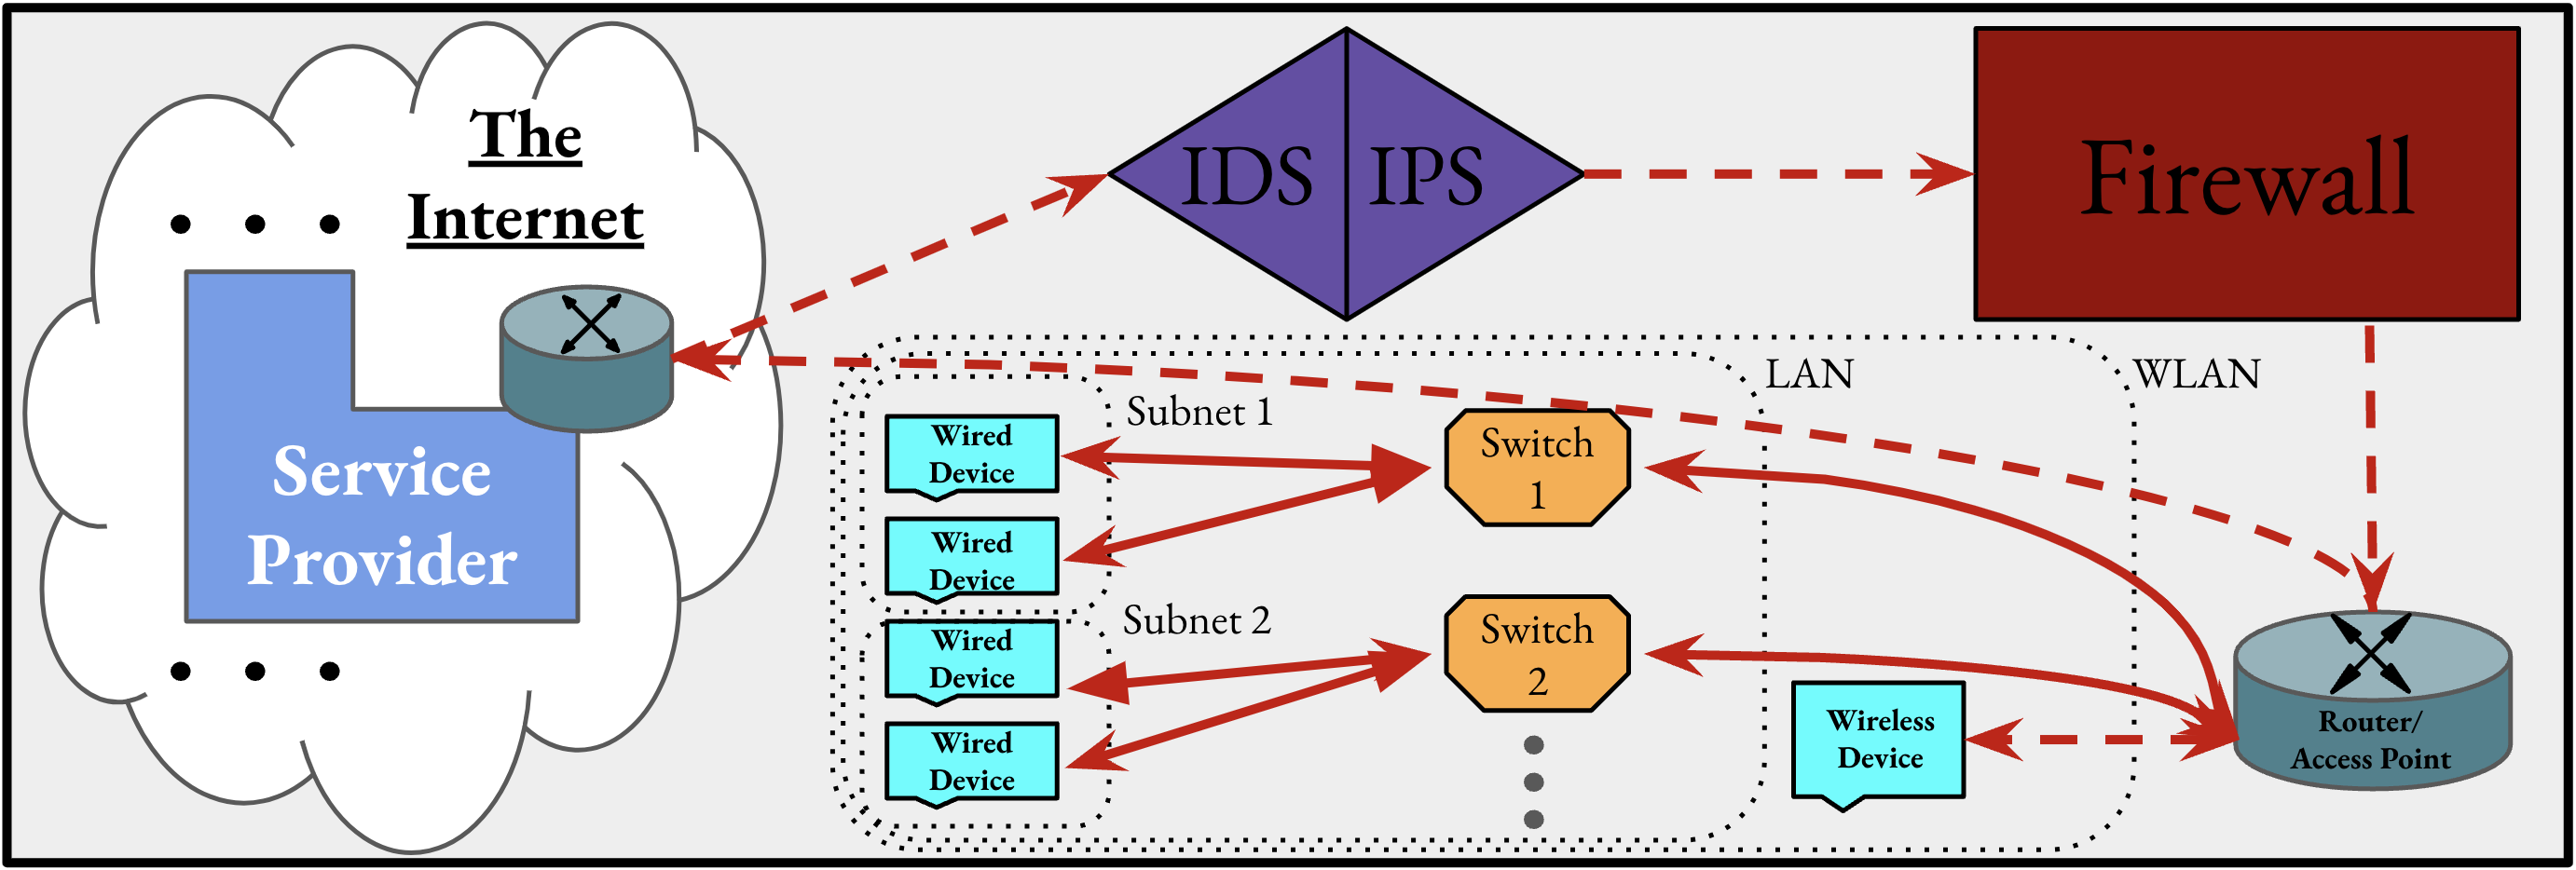
\includegraphics[width = 15.55cm, height = 6.05cm]{Network.png}
    \end{center}
    \vspace{0.5em}
\end{orangebox}

\begin{center}
    \vspace{-0.25em}
    \hspace{0.2cm}\pgfornament[color=orange,width=1cm,ydelta=-10pt]{11}\pgfornament[color=orange,width=0.5cm,ydelta=-10pt]{6}\pgfornament[color=orange,width=1cm,ydelta=-10pt]{14}
    \vspace{-0.4em}
\end{center}

\begin{orangebox}{Tuesday, June 6th\vspace{-2.2em}\begin{flushright}\large\textbf{UTM (new VM) \& Suricata} \emoji{penguin}\emoji{hamster}\end{flushright}}
    \begin{itemize}
        \item \texttt{multipass} is becoming more trouble than it's worth; when trying to launch a shell from the primary (or any) instance, it takes forever and times out. Other people seem to have similar problems: see Issues tab of the \texttt{multipass} \href{https://github.com/canonical/multipass/issues}{\textbf{GitHub repo}}. I suspect this is because of my M1 Mac, so I've looked into what people recommend and found \href{https://mac.getutm.app/}{\textbf{UTM}} as a possible alternative for a Linux VM. Installation steps:
        \begin{itemize}
            \item Install \href{https://cdimage.ubuntu.com/jammy/daily-live/current/}{\texttt{Ubuntu 22.04}}, choosing the \textbf{64-bit ARM (ARMv8/AArch64)} desktop image option instead of the AMD option for this Mac's M1 processor. This will produce a \texttt{jammy-desktop-arm64.iso}, which you can save anywhere (desktop).
            \item Follow \href{https://www.youtube.com/watch?v=1WWj6qoWhJw}{\textbf{this video's}} instructions to install \href{https://mac.getutm.app/}{\textbf{UTM}}.
            \item In the VM, follow \href{https://www.digitalocean.com/community/tutorials/how-to-install-suricata-on-ubuntu-20-04}{\textbf{this guide}} to install \href{https://en.wikipedia.org/wiki/Suricata_(software)}{\textbf{Suricata}}, an open-source based IDS/IPS.
        \end{itemize}
        \item \textbf{Today's Assignment:} You should research how to test a rule against a PCAP file after you install Suricata in Linux, not configuring the whole utility as a daemonized service and leaving it running long-term. You will only need to do the former.
        \begin{enumerate}
            \item You've been alerted that \codebox{27.43.100.29} is on a threat list targeting web services. Write a signature that alerts on accesses from this host to any local web service.
            \item Your organization recently noticed that malicious actors were scanning for \codebox{phpMyAdmin} at \codebox{/phpMyAdmin/scripts/setup.php} on our web servers. The scan engine did not set a User-Agent. Write an alert for whenever an external host tries to fetch that URI without a User-Agent set. Test with \codebox{http.pcapDownload http.pcap}.
            \item A few years ago a phishing attack was launched where the attacker got multiple users to add a malicious service as a trusted service on their Google account. The attack required the victim to click on a link to \href{https://accounts.google.com/o/oauth2/auth}{\codebox{https://accounts.google.com/o/oauth2/auth}}. Write a signature that finds all email with a link to that address. Test with \codebox{smtp.pcapDownload smtp.pcap}.
            \item You are looking for data inside the friends lists on Yahoo! Messenger packets. The protocol is documented here: \href{http://libyahoo2.sourceforge.net/ymsg-9.txt}{\codebox{http://libyahoo2.sourceforge.net/ymsg-9.txt}}. Write a rule that will identify Yahoo messenger packets with a service of \codebox{00 f1} (this replaced \texttt{YAHOO\_SERVICE\_LIST} at some undocumented point in ancient history). You can test this against \codebox{ymsg2.pcap Download ymsg2.pcap}.
        \end{enumerate}
    \end{itemize}
\end{orangebox}

\begin{center}
    \vspace{-0.25em}
    \hspace{0.2cm}\pgfornament[color=orange,width=1cm,ydelta=-10pt]{11}\pgfornament[color=orange,width=0.5cm,ydelta=-10pt]{6}\pgfornament[color=orange,width=1cm,ydelta=-10pt]{14}
    \vspace{-0.4em}
\end{center}

\begin{orangebox}{Wednesday, June 7th\vspace{-2.2em}\begin{flushright}\large\textbf{UTM \& Suricata, Continued} \emoji{hamster}\emoji{counterclockwise-arrows-button}\end{flushright}}
    \begin{itemize}
        \item Beginning where we left off yesterday, the first necessary step is to set up file sharing between the host and guest machines. For UTM, this will make use of the SPICE WebDAV directory share mode, which which you can access a selected shared directory:
        \begin{enumerate}
            \item Following \href{https://docs.getutm.app/guest-support/linux/}{\textbf{these instructions}}, ensure that the SPICE agent is installed. The SPICE agent is required for clipboard sharing (both QEMU and Apple backend) as well as dynamic display resolution in QEMU backend. Run these commands: \\
            \codebox{\$ sudo apt install spice-vdagent} \codebox{\$ sudo apt install qemu-guest-agent}
            \item Install the SPICE WebDAV with \codebox{\$ sudo apt install spice-webdavd}. 
            \item Ensure no virtual machines are running, and open UTM. Select the desired VM, then click the top-rightmost icon in the window. Now, we are in \codebox{Settings $>$ Sharing $>$ Directory Share Mode}. Select \texttt{SPICE WebDAV}. Also ensure that the box above it is checked to enable clipboard sharing. Below it is a path where the shared directory folder with the \texttt{.pcap} files can be selected.
            \item Then, you should be able to access \codebox{http://127.0.0.1:9843} from a browser inside the guest machine once it is running. This will render an HTML view of the shared directory folder that was manually selected in the previous step. You may click through the hyperlinks and click on the files to download them. \\
            \textbf{Note:} a \href{https://github.com/utmapp/UTM/discussions/3917}{\textbf{common bug}} where the VM's \texttt{Spice client tools} folder can't open.
        \end{enumerate}
        \item Continuing with yesterday's assignment, question 1 asks to write a signature that alerts on accesses from to any local web services, with \codebox{27.43.100.29}being on a threat list:
    \end{itemize}
    \switchuser{host=amalysz@ubuntum1, prompt char=\textcolor{ubuntublue}{/Desktop}}
    \begin{ubuntu}
$ pwd `\BeginConsole`
/home/amalysz/Desktop `\switchuser{host=amalysz@ubuntum1, prompt char=\textcolor{ubuntublue}{/Desktop}}`
$ ls `\BeginConsole`
eve.json  fast.log  http.pcap  smtp.pcap  stats.log  suricata.log  ymsg2.pcap`\switchuser{host=amalysz@ubuntum1, prompt char=\textcolor{ubuntublue}{/Desktop}}`
$ ls -lh `\BeginConsole`
total 148K
-rw-r--r-- 1 root    root     70K Jun  7 13:40 eve.json
-rw-r--r-- 1 root    root    1.4K Jun  7 13:40 fast.log
-rw-rw-r-- 1 amalysz amalysz 1.9K Jun  7 12:23 http.pcap
-rw-rw-r-- 1 amalysz amalysz 5.2K Jun  7 12:25 smtp.pcap
-rw-r--r-- 1 root    root     21K Jun  7 13:40 stats.log
-rw-r--r-- 1 root    root     13K Jun  7 13:40 suricata.log
-rw-rw-r-- 1 amalysz amalysz 9.9K Jun  7 12:25 ymsg2.pcap `\switchuser{host=amalysz@ubuntum1, prompt char=\textcolor{ubuntublue}{/Desktop}}`
$ cd /var/lib/suricata
    \end{ubuntu}
\end{orangebox}

\begin{orangebox}{Wednesday, June 7th \hspace{0.2cm}(cont. \#1/1)\vspace{-2.2em}\begin{flushright}\large \emoji{hamster}\emoji{counterclockwise-arrows-button}\end{flushright}}
    \switchuser{host=amalysz@ubuntum1, prompt char=\textcolor{ubuntublue}{/var/lib/suricata}}
    \begin{ubuntu}
$ ls`\BeginConsole`
rules update`\switchuser{host=amalysz@ubuntum1, prompt char=\textcolor{ubuntublue}{/var/lib/suricata}}`
$ sudo nano custom-rules.rules
    \end{ubuntu}
    \begin{itemize}
        \item \textbf{Note:} The reason we \codebox{cd} into \codebox{/var/lib/suricata} is because that is the default rule path for configuring Suricata to load Suricata-Update managed rules, as we can find by \codebox{cd}-ing into \codebox{cd /etc/suricata}, opening \codebox{open suricata.yaml}, and finally searching for the \codebox{rule-files:} config directive, as below:
    \end{itemize}
    \begin{center}
        \vspace{-0.5em}
        \phantom{~~~~~~~}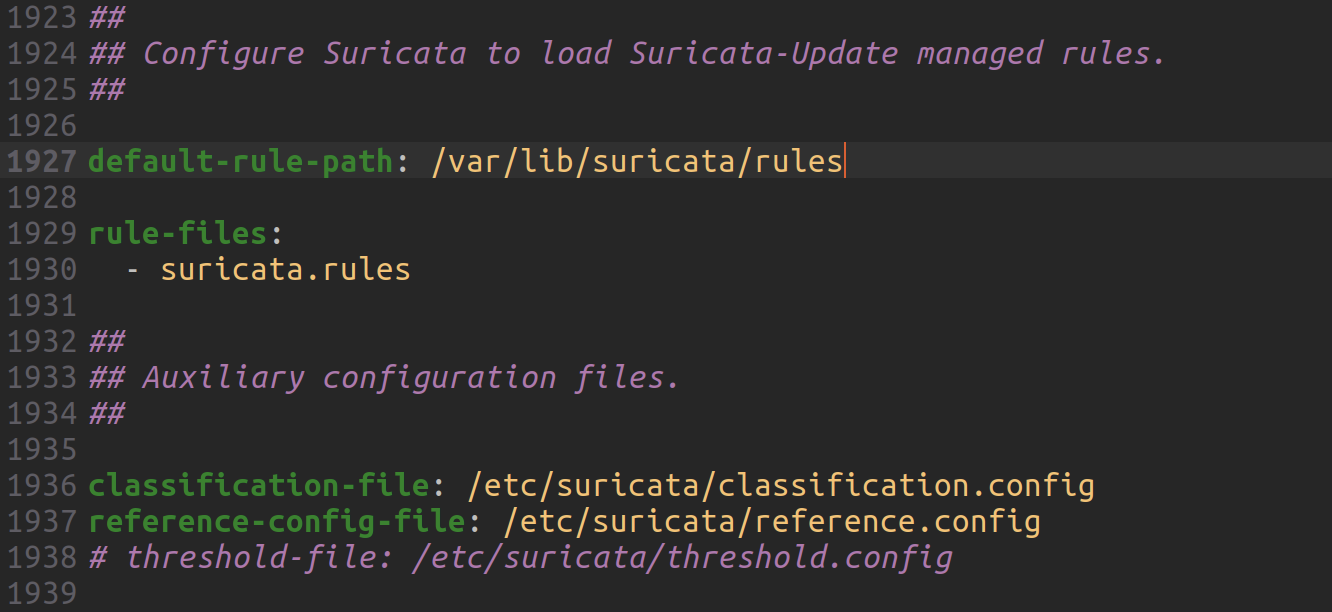
\includegraphics[width = 14.4cm, height = 6cm]{suricata.yaml screenshot.png}
    \end{center}
    \begin{itemize}
        \vspace{-1.75em}
        \item Write and \href{https://asciinema.org/a/488029}{\textbf{test}} four custom Suricata rules in \texttt{custom-rules.rules} using its \href{https://www.youtube.com/watch?v=d-t-8lJ2PII&t=829s}{\textbf{syntax}}.\\
        \textbf{Note:} pre-set labels like \texttt{\$HOME\_NET} and \texttt{\$EXTERNAL\_NET} are in \texttt{<some file>}, where custom labels can also be configured for individual/ranges of IPs, including ports:
    \end{itemize}
    \switchuser{host=amalysz@ubuntum1, prompt char=\textcolor{ubuntublue}{/var/lib/suricata}}
    \begin{ubuntu}
$ sudo nano custom-rules.rules`\BeginConsole`
alert http 27.43.100.29 any -> $HOME_NET any (msg:"threat list"; flow:to_server; sid:1; rev:1;)
alert http any any -> $HOME_NET$ any (msg:"phpMyAdmin scan"; flow:established,to_server; content:"GET"; http_uri:"/phpMyAdmin/scripts/setup.php"; http_header:!"User-Agent"; sid:2; rev:2;)
alert smtp any any -> $HOME_NET any (msg:"phishing"; flow:to_server; content:"https://accounts.google.com/o/oauth2/auth"; sid:3; rev:3;)
alert tcp any any -> $HOME_NET any (msg:"Yahoo"; content:"|59 4d 53 47 00 13 00 00|"; content:"|00 f1|"; distance:2; within:4; sid:4; rev:4;)
    \end{ubuntu}
\end{orangebox}

\begin{center}
    \vspace{-0.25em}
    \hspace{0.2cm}\pgfornament[color=orange,width=1cm,ydelta=-10pt]{11}\pgfornament[color=orange,width=0.5cm,ydelta=-10pt]{6}\pgfornament[color=orange,width=1cm,ydelta=-10pt]{14}
    \vspace{-0.4em}
\end{center}

\normalsize\begin{orangebox}{Thursday, June 8th\vspace{-2.2em}\begin{flushright}\large Q\&A with VPNs \emoji{detective}\emoji{exclamation-question-mark}\end{flushright}}
    \begin{itemize}
        \item\textbf{What is the basic premise of a VPN?} \\
        \phantom{~~~~} VPN means ``virtual private network". VPN services will pass your data through their VPN client downloaded onto your device instead of going directly to your ISP from your modem---this is to encrypt the traffic from third parties. It then goes from them to your VPN server, and from there to the internet. This last step allows you to configure your appeared location, as companies have VPN servers all over the world.
        \item\textbf{How does a VPN's cryptography work? Do you retain total anonymity?} \\
        \phantom{~~~~} When the VPN client and VPN server initiate a connection, they must authenticate each other and establish an encrypted tunnel. Authentication methods are usually... \\
        \phantom{~~~~} Pre-shared keys are exchanged by both client and server as a means of mutual authentication to initiate the tunneling protocol: this begs the question of how sharing of said keys is secure in the first place, and may take place such that each downloaded client comes with a unique key and a key to expect from the server (or, these passwords may be exchanged via encrypted traffic over the network). \\
        \phantom{~~~~} Certificates are the better-scaling option, but they need to be purchased and issued from the CA (Certificate Authority). They contain the public key for a digital signature and specifies the identity associated with the key, such as the name of an organization. The certificate is used to confirm that the public key belongs to said organization. \\
        \phantom{~~~~} Privacy and anonymity are often confused services that a VPN provides, which only includes the former. When intercepting traffic from a VPN or attempting to keep logs of it as an ISP, packet contents are encrypted, but meta data such as source/destination ports, the VPN's IP address(es), number and frequency of connections, amount of data transferred, etc. will always remain visible. Profiles can be built around this meta data to associate with individual devices. The VPN services still remain useful, though.
        \item\textbf{Like with overlay of security protocols, how can multiple services be using the same port(s) simultaneously? How many ports are there?} \\
        \phantom{~~~~} To some degree of abstraction, ports are just reserved lines of communication that can be recognized by a sender and receiver, and they shouldn't be thought of as physical space residing anywhere. For reasons that ``seemed to be correct at the time," ports are assigned 16-bits each in the header blocks of each TCP and UDP packet---in total, 32-bits. This means $2^{16}-1=65535$ possible ports to be used at any given time. The reason a port can receive multiple communications simultaneously is because of the different sender port labels: they're just a way for the computer to keep ongoing conversations separate, and for said lines to know when to be expecting answers.
    \end{itemize}
\end{orangebox}

\begin{orangebox}{Thursday, June 8th \hspace{0.2cm}(cont. \#1/2)\vspace{-2.2em}\begin{flushright}\emoji{detective}\emoji{exclamation-question-mark}\end{flushright}}
    \begin{itemize}
        \item\textbf{Is it more secure to run SSH through a non-default port? How can someone find out an SSH service is running on any port without prior knowledge?} \\
        \phantom{~~~~} By running SSH through a non-default port, you prevent communication from all sources that know to look for it, and lower the scope of sources that can contact the server. This filters false-malicious connections to a minimum from scripted attacks, meaning repeated failed connection requests suggest the server is being targeted. This also means that any automated or trusted sources that know to look for the default port must also be informed, however. \\
        \phantom{~~~~} Taken from this \href{https://unix.stackexchange.com/questions/539882/find-which-port-does-ssh-client-used-to-send-connection-request}{\textbf{source}}, to know what port a particular ssh connection will use, you can look in \codebox{/etc/ssh/ssh\_config} for any system/global hosts configured, and in \codebox{~/.ssh/config} for any user/local hosts. To know what port will be used by default, you can use the command \codebox{\$ getent services ssh} (the standard port is 22). To know what ports are actively in use, the command \codebox{\$ netstat --tcp --programs --numeric | grep ssh} should show you.
        \item\textbf{What are the VPN protocols IPSec, OpenVPN, and Wireguard?} \\
        \phantom{~~~~} Where IP is the standard that says how and where data should go over the internet, IPsecure adds encryption and authentication on top of that process to avoid unwanted monitoring of network traffic; it scrambles information at the source and unscrambles information at the destination. IPsec connections are commonly used with VPNs when accessing files remotely, for example (like with NIST). \\
        \phantom{~~~~} OpenVPN is an open-sourced VPN protocol integrated into a lot of commercial VPNs' models. It uses UDP primarily for the sake of having fast connections---some of which are across the world streaming video, so speed is more of the essence (and if data is scrambled on top as a security measure, packet order won't make a difference and neither will dropping a handful of them in comparison)---but also supports TCP connections as a backup option. \\
        \phantom{~~~~} Wireguard is a third free, open-sourced tunneling protocol that uses only UDP with the goal of improved performance over the aforementioned two. It's also said to be fast because its low-level components are built into the Linux kernel, making it faster than userspace VPNs. It launched in 2015 with newer and faster cryptographic methods, also focusing on minimizing attack surface against hackers. It does not counter deep-packet inspection alone, however, but has the architecture to support further obfuscation.
    \end{itemize}
    \begin{center}
        \vspace{-0.5em}
        \large\bullet \\
        \large\bullet \\
        \large\bullet \\
        \Large\textbf{(\textit{Continued...})}
    \end{center}
\end{orangebox}

\begin{orangebox}{Thursday, June 8th \hspace{0.2cm}(cont. \#2/2)\vspace{-2.2em}\begin{flushright}\emoji{detective}\emoji{exclamation-question-mark}\end{flushright}}
    \begin{itemize}
        \item\textbf{How does a VPN client (say, Ubuntu Linux) know to not leak data by sending traffic outside the VPN (through the normal network connection)?}
        \begin{enumerate}
            \item\textbf{Routing:} Upon establishing a connection, the VPN client modifies the routing table on the OS, adding a route that directs all traffic through the VPN tunnel.
            \item\textbf{Network Firewall:} The VPN client may also employ a network firewall to block any outgoing network connections that are not intended to go through the VPN tunnel. The firewall rules are set up to allow only the VPN traffic to pass through.
            \item\textbf{DNS Leak Protection:} DNS (Domain Name System) leak is a common issue where DNS requests made by the operating system bypass the VPN tunnel and are resolved by the default DNS servers of the network. To prevent this, the VPN client typically configures the system to use its own DNS servers.
            \item\textbf{Kill Switch:} A kill switch is a fail-safe that monitors the VPN connection status and immediately blocks all network traffic if the VPN connection drops unexpectedly, preventing any data from being transmitted outside the VPN tunnel.
        \end{enumerate}
        \item\textbf{How could you tell that someone is using a VPN, and how could you hide that fact from someone else?} \\
        \phantom{~~~~} An ISP logs the data of its users, and when it expects to read that data and finds that it's encrypted upon arrival, then it knows a VPN is being used---this is true for anyone intercepting traffic from the (W)LAN to the ISP. The solution is to hide the packets in plain sight, disguising their contents as something else that \textit{is} readable. A real-life motivation for disguising a VPN is in countries where VPNs are illegal. The scope of IP addresses should also be taken into consideration, as some entire countries may even share (a small range of) them.
        \item\textbf{Looking for meta data---even surrounding encrypted packet contents---is a standard practice; how could someone use cryptography to apply a further layer of security and hide that meta data?} \\
        \phantom{~~~~} The concept of analyzing meta data hinges on the fact that said data is truthful, meaning said user's actions are uninfluenced by surveillance. If someone were to apply noise to this meta data by sending garbage packets randomly in the mix, the data becomes harder to extrapolate. For instance, a second layer of meta-security could be enforced where packets are send along a TCP stream along with garbage packets: the real packets are encrypted by the usual encrypted tunneling, but the garbage packets' placement is well-ordered and adheres to an additional pre-exchanged sequence (e.g. the real packets' indices in the stream correspond to Fibonacci numbers).
    \end{itemize}
\end{orangebox}

\begin{center}
    \vspace{-0.25em}
    \hspace{0.2cm}\pgfornament[color=orange,width=1cm,ydelta=-10pt]{11}\pgfornament[color=orange,width=0.5cm,ydelta=-10pt]{6}\pgfornament[color=orange,width=1cm,ydelta=-10pt]{14}
    \vspace{-0.4em}
\end{center}

\normalsize\begin{orangebox}{Friday, June 9th\vspace{-2.2em}\begin{flushright}VPN Lab with AWS \emoji{microscope}\emoji{cloud}\end{flushright}}
    \begin{itemize}
        \item Today's agenda will be to perform a VPN lab. We will buy digital infrastructure from AWS to run a server that we will communicate with using OpenVPN, in order to observe how it encapsulates packets. The goal will be to SSH into the server using our remote machine (Ubuntu Linux VM), capture that traffic on our host machine in the form of a \texttt{.pcap} file using \texttt{tcpdump}, and finally examine said file using Wireshark:
        \begin{enumerate}
            \item Accept an invitation to create an account with \href{https://en.wikipedia.org/wiki/Okta,_Inc.}{\textbf{Okta}} (an American identity and access management company), which will allow AJ to add you to an AWS account \texttt{surf-vpn-research} that can be accessed from the Okta dashboard.
            \item Visit the Console Home of \texttt{surf-vpn-research}, and then go to the EC2 tab (Elastic Control Cloud allows users to rent virtual computers on which to run their own computer applications).
            \item Select the running instance \texttt{openvpn-test}, and click ``Connect"; in the connection options, select the Session Manager tab to enable SSH connections to the server.
            \item As long as the server is running, ideally you should be able to ssh into the server on the Ubuntu Linux VM's console; however, we experienced some trouble with this, and will try again on Monday. Instead, we can SSH into the server on our Mac's terminal with the server's IP address: \codebox{ssh ssm-user@54.211.93.59}. \\
            \textbf{Note:} at this point, the server is configured to only allow connections over two ports from public Internet: TCP/22 for SSH and TCP/443 for OpenVPN TCP.
            \item Following this \href{https://www.comparitech.com/net-admin/tcpdump-capture-wireshark/}{\textbf{guide}}, first ensure that \texttt{tcpdump} is installed by running \codebox{\$ brew install tcpdump} in a separate terminal.
            \item After SSH-ing into the server, run \codebox{\$ sudo tcpdump -s 0 -i eth0 -w tcpdump.pcap} to begin capturing traffic with \texttt{tcpdump}. You may let it run for about a minute or two (or until you've done something you'd like to examine while collecting traffic) before ending the session with \codebox{Ctrl+C}.
            \item Before you can copy the traffic from (what should be) your remote computer to the local one for analysis with Wireshark, you’ll have to change the permissions. By default, \texttt{tcpdump} sessions captured by the root user can’t be copied. Change this by running \codebox{\$ sudo chmod 644 tcpdump.pcap}.
            \item To copy the new file \texttt{tcpdump.pcap} to the host machine, run \codebox{\$ scp ssm-user@54.211.93.59:home/ssm-user/tcpdump.pcap .\textbackslash}. \\
        \end{enumerate}
        \vspace{-1.5em}
        The \texttt{.pcap} file can now be opened and analyzed with Wireshark on the host computer.
    \end{itemize}
\end{orangebox}

\newpage

\noindent\begin{longfbox}[
    rounded,
    padding=4pt,
    border-width=1.5pt,
    border-top-left-radius=30pt,
    border-left-width=8pt,
    border-color=shininggold,
    background-color=Lshininggold,
    border-right-style=double,
]
    \medskip
    \phantom{~~}\Large\textbf{WEEK \barroman{IV}.} \large(06/12 - 06/16)\phantom{~~~~~~~~~~~~~~~~~~~~~~~~~~~~~~~~~~~~~~~~~~~~~~~~~~~~~~~~~~~~~~~~~~~~~~~~~~~~~~~~}
\end{longfbox}
\\

\begin{center}
    \vspace{-1em}
    \hspace{0.1cm}\pgfornament[color=shininggold, width=6cm, ydelta=-10pt]{88}
    \vspace{-0.5em}
\end{center}

\begin{shininggoldbox}{Monday, June 12th\vspace{-2.2em}\begin{flushright}\large PCAP Expressions \emoji{candy}\emoji{pencil}\end{flushright}}
    \begin{multicols}{2}
        \Large\textbf{\textit{\underline{What we talk about when we}}} \\ 
        \Large\textbf{\textit{\underline{talk about pcap expressions}}}
        \bigskip
        
        \normalsize Nik Sultana, University of Pennsylvania
        \columnbreak
        \begin{mdframed}
        \tiny Nik Sultana. 2019. What we talk about when we talk about pcap expressions. In Real World Domain Specific Languages (RWDSL), February 17, 2019, Washington D. C., DC, USA. ACM, New York, NY, USA, 9 pages. \\ https://doi.org/10.1145/nnnnnnn.nnnnnnn
        \end{mdframed}
        \vspace{-2em}
    \end{multicols}
    \vspace{-2em}
    \textbf{\hline}
    \begin{itemize}
        \item\textbf{BSD Packet Filter (BPF - Berkeley Packet Filter)} : PCAP :: Assembly : C
        \vspace{-0.5em}
        \begin{itemize}
            \item The most successful host-based system for capturing network packets.
            \item Included in the \texttt{libpcap} library, the basis for \texttt{tcpdump}.
            \item BPF is in the form of instructions for a VM, which are compiled into machine code by a just-in-time (JIT) mechanism and executed in the kernel to reduce overhead from userspace-kernel transitions (see below).
        \end{itemize}
        \vspace{-0.75em}
        \item These filters form a domain-specific language (DSL) called ``\textbf{PCAP expressions}''.
        \vspace{-0.75em}
        \item These are either fed to IDS/IPS or can be exported as \texttt{.pcap} files for offline analysis.
        \vspace{0.25em}
    \end{itemize}
    \vspace{-3em}
    \begin{center}
        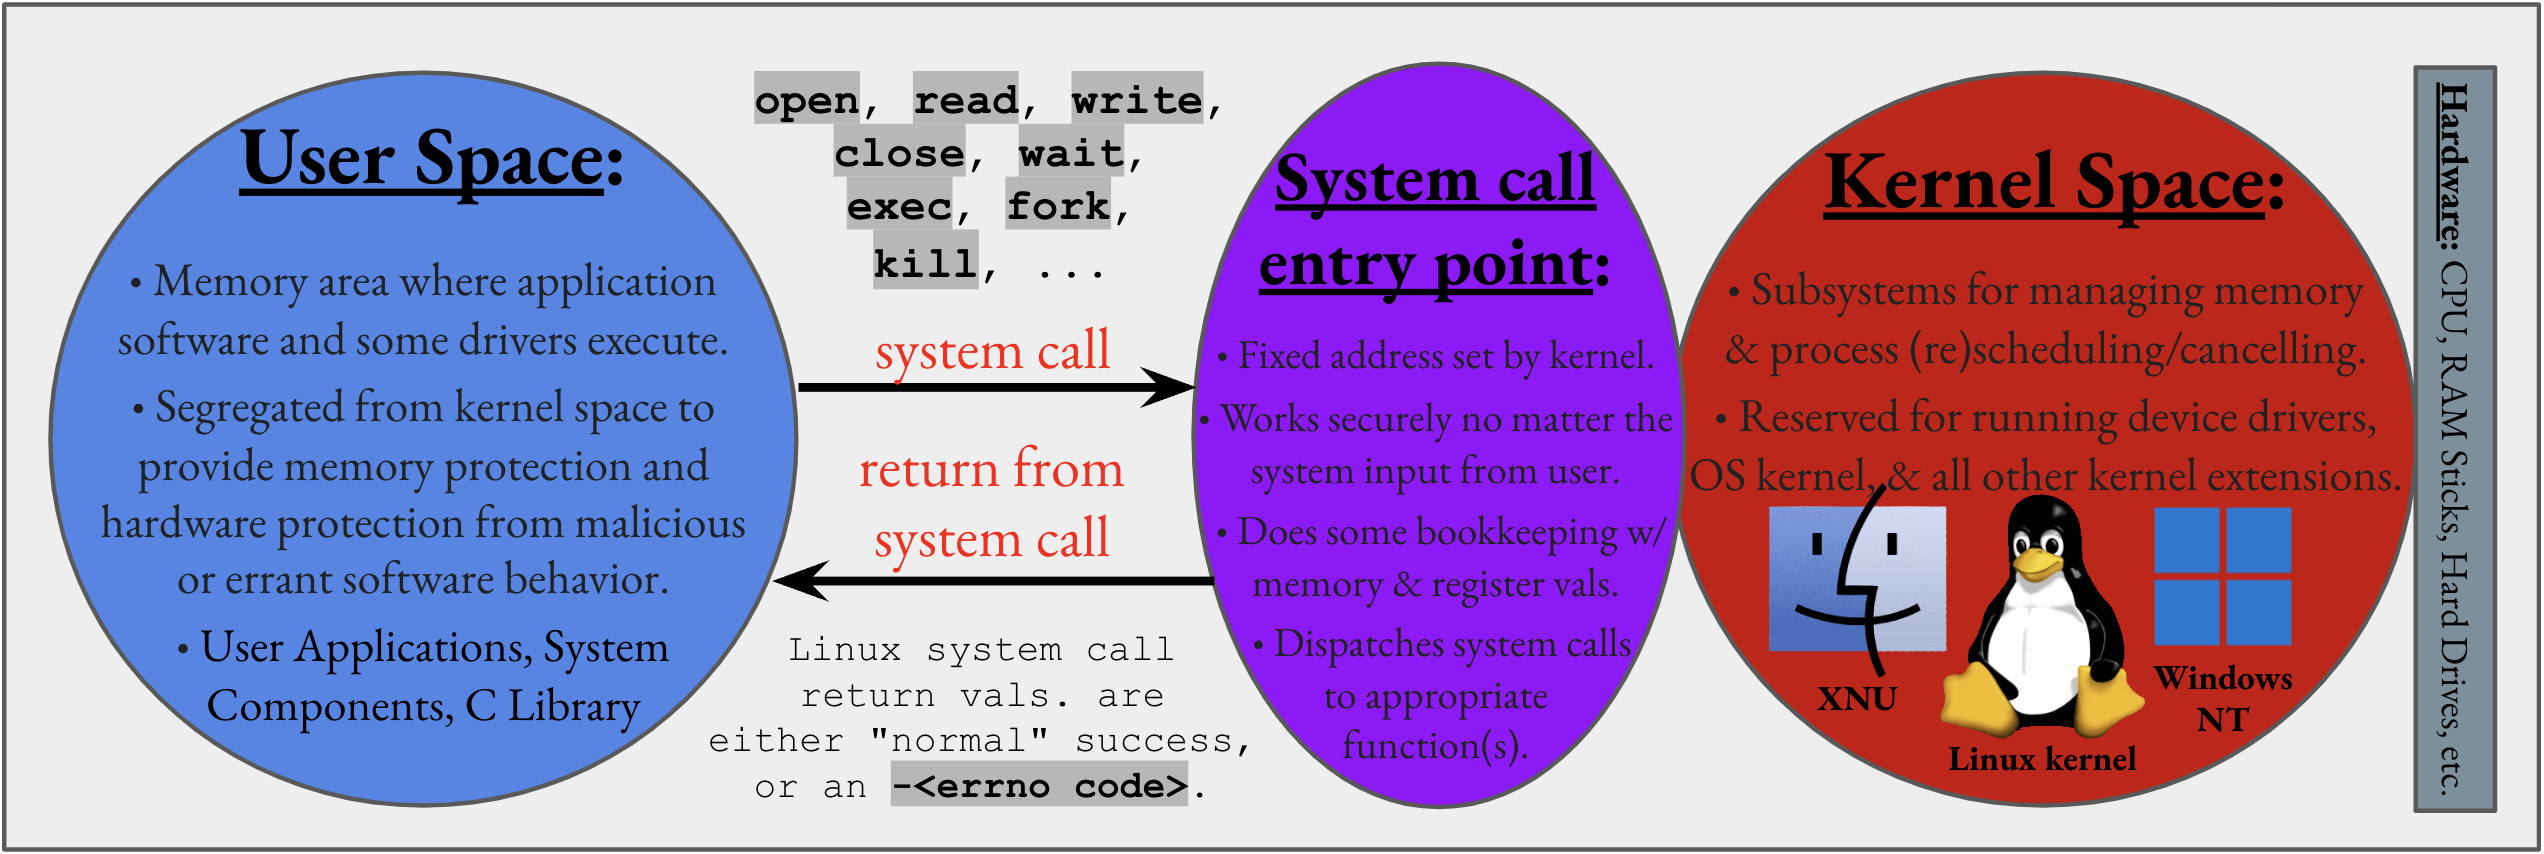
\includegraphics[width = 15.5cm, height = 5cm]{User and Kernel Space.png}
    \end{center}
    \vspace{-2em}
    \begin{itemize}
        \item\href{https://gitlab.com/niksu/caper}{\textbf{Caper}} is a free open-source language provided with the formal semantics of the PCAP expression language to act as an equivalence-checker tool.
        \vspace{-0.75em}
        \begin{itemize}
            \item It can emit warnings for queries with unexpected behaviors, such as non-isomorphic permutations of clauses that lead to subsumations (see below).
            \item It implements a parser for the full PCAP language and its semantics to expand them into equivalent PCAP expressions.
            \item These can then be fed to \textbf{SMT solvers}, which are like SAT Solvers except generalized to mathematical formulae instead of just boolean statements.
            \item Equivalences are determined using bit-vector semantics (see Figs. 1-3).
        \end{itemize}
    \end{itemize}
\end{shininggoldbox}

\begin{center}
    \vspace{-0.25em}
    \hspace{0.2cm}\pgfornament[color=shininggold,width=1cm,ydelta=-10pt]{11}\pgfornament[color=shininggold,width=0.5cm,ydelta=-10pt]{6}\pgfornament[color=shininggold,width=1cm,ydelta=-10pt]{14}
    \vspace{-0.4em}
\end{center}

\begin{shininggoldbox}{Tuesday, June 13th\vspace{-2.2em}\begin{flushright}\large PCAP Literature \emoji{candy}\emoji{glasses}\end{flushright}}
    \begin{multicols}{2}
        \large\textbf{\textit{\underline{The BSD Packet Filter:}}} \\ 
        \large\textbf{\textit{\underline{A New Architecture for User-level}}} \\
        \large\textbf{\textit{\underline{Packet Capture}}}
        \bigskip
        
        \normalsize Steven McCanne \& Van Jacobson, \\
        Lawrence Berkeley Laboratory
        \columnbreak
        \begin{mdframed}
            \tiny McCanne, S., Jacobson, V. 1993. The BSD Packet Filter: A New Architecture for User-level Packet Capture. In Proceedings of the 1993 Winter USENIX Conference (January 25-29, 1993, San Diego, CA). Preprint version. Lawrence Berkeley Laboratory, Berkeley, CA. Technical Report No. LBL-33878. December 19, 1992. Supported by the Director, Office of Energy Research, Scientific Computing Staff, U.S. Department of Energy, Contract No. DE-AC03-76SF00098.
        \end{mdframed}
        \vspace{-2em}
    \end{multicols}
    \vspace{-2em}
    \textbf{\hline}
    \begin{itemize}
        \normalsize\item\textbf{BSD Packet Filter (BPF - Berkeley Packet Filter)} : PCAP :: Assembly : C
        \vspace{-0.25em}
        \item This paper is likely more involved in eBPF than PCAP expressions for our purposes.
    \end{itemize}
\end{shininggoldbox}

\begin{center}
    \vspace{-0.25em}
    \hspace{0.2cm}\pgfornament[color=shininggold,width=1cm,ydelta=-10pt]{11}\pgfornament[color=shininggold,width=0.5cm,ydelta=-10pt]{6}\pgfornament[color=shininggold,width=1cm,ydelta=-10pt]{14}
    \vspace{-0.4em}
\end{center}

\begin{shininggoldbox}{Wednesday, June 14th\vspace{-2.2em}\begin{flushright}\large PCAP Translators \emoji{candy}\emoji{japanese-congratulations-button}\end{flushright}}
    \begin{itemize}         
        \item There is a production team behind \href{https://github.com/the-tcpdump-group/tcpdump/tree/master}{\textbf{tcpdump}} and \href{https://github.com/the-tcpdump-group/libpcap/tree/master}{\textbf{libpcap}}---a powerful command-line packet analyzer and a portable C/C++ library for network traffic capture, respectively---that have produced a tool called \href{https://www.tcpdump.org/bpfexam/}\textbf{BPFExam}; essentially, borrowing some features from Professor Sultana's project \href{https://gitlab.com/niksu/caper}{\textbf{Caper}} (which we reviewed a few days ago) to provide the caper expansion and caper translation from PCAP to English, and also from PCAP to bytecode accessible by the OS kernel.
        \vspace{-0.25em}
        \begin{itemize}
            \item Ideally, the tool we are building should be able to do the reverse: take an English expression of the format translated by BPFExam, and translate it into a PCAP expression. This would obviously never include all free-form English, but rather a formatted version of it---perhaps including artificial symbols to parse clauses, etc.
            \item In addition to its functionality as a translator from English to PCAP, our project should likewise rely on some frontend web development like Caper; this will at some point require some research into web frameworks that integrate OCaml, if they exist at all. I suspect the backend would bee too ambitious in scope.
        \end{itemize}
        \vspace{-0.5em}
        \item Without getting too much ahead of ourselves, we would need to keep in mind a ``zero-trust'' policy of user-input into our program; not only to produce the intended output correctly, but for possible security concerns regarding injection attacks. We can calm it down to simple phrases, and maybe we can define keywords like ``workstation network" and ``Internet" depending on a provided definition? I suspect this would work like an OCaml interpreter would, using a substitution environment and defining these words in various dictionaries. Everything should cater towards \href{https://en.wikipedia.org/wiki/Behavior-driven_development#Behavioral_specifications}{\textbf{Behavior-Driven-Development (BDD)}}, or ``customer representatives" who would use the product.
    \end{itemize}
\end{shininggoldbox}

\begin{center}
    \vspace{-0.25em}
    \hspace{0.2cm}\pgfornament[color=shininggold,width=1cm,ydelta=-10pt]{11}\pgfornament[color=shininggold,width=0.5cm,ydelta=-10pt]{6}\pgfornament[color=shininggold,width=1cm,ydelta=-10pt]{14}
    \vspace{-0.4em}
\end{center}

\begin{shininggoldbox}{Thursday, June 15th\vspace{-2.2em}\begin{flushright}\large Building Expressions \emoji{candy}\emoji{construction-worker}\end{flushright}}
    \begin{itemize}         
        \item Tried my hand at manually translating English network policy into PCAP expressions:
        \vspace{-2em}
        \begin{itemize}
            \item ``The organization should only allow DNS traffic for all staff workstation networks to the approved internal DNS service." $\Longrightarrow$ \\
            \hspace{-2cm}\codebox{dst port 53 and (src net <work\_net> or dst net <work\_net>)}
            \item ``The organization should only allow web traffic from all staff workstation networks to the public Internet from the organization's web proxy service." $\Longrightarrow$ \\
            \codebox{(dst port 80 or dst port 443) and src net <staff\_net> and} ... \\
            ... \codebox{dst net <public\_net> and src host <web\_proxy>}
            \item ``The organization should not allow any VPN traffic from the inside all staff workstation networks to the public Internet." $\Longrightarrow$ \\
            \codebox{not (src net <staff\_net> and dst net <public\_net> and} ... \\
            ... \codebox{(src port <vpn\_port> or dst port <vpn\_port>))}
            \item ``The organization's web traffic from all staff workstations network through the organization's web proxy service (VPN). These workstations should not be able to visit any of the following websites in the list \texttt{prohib\_list = [www.foo.com, www.bar.com, www.zoo.com]}." $\Longrightarrow$ \\
            \codebox{src net <staff\_net> and dst net <public\_net> and src host <web\_proxy> and}
            \codebox{not (dst host www.foo.com or dst host www.bar.com or dst host www.zoo.com)}
        \end{itemize}
        \vspace{-2em}
        \item Drew up a \href{https://docs.google.com/document/d/1hRBz8IYQxX02fCSRM8ljHqrv7i1HLet6dXB-_NdKSJY/edit?usp=sharing}{\textbf{rough outline}} of our project's soon-to-be substitution algorithm in GDocs.
    \end{itemize}
\end{shininggoldbox}

\begin{center}
    \vspace{-0.25em}
    \hspace{0.2cm}\pgfornament[color=shininggold,width=1cm,ydelta=-10pt]{11}\pgfornament[color=shininggold,width=0.5cm,ydelta=-10pt]{6}\pgfornament[color=shininggold,width=1cm,ydelta=-10pt]{14}
    \vspace{-0.4em}
\end{center}

\begin{shininggoldbox}{Friday, June 16th}
    \begin{itemize}         
        \item This is my own box with a mandatory title.     
    \end{itemize}
\end{shininggoldbox}
\newpage

\noindent\begin{longfbox}[
    rounded,
    padding=4pt,
    border-width=1.5pt,
    border-top-left-radius=30pt,
    border-left-width=8pt,
    border-color=yellow,
    background-color=Lyellow,
    border-right-style=double,
]

    \medskip
    
    \phantom{~~}\Large\textbf{WEEK \barroman{V}.} \large(06/19 - 06/23)\phantom{~~~~~~~~~~~~~~~~~~~~~~~~~~~~~~~~~~~~~~~~~~~~~~~~~~~~~~~~~~~~~~~~~~~~~~~~~~~~~~~~}
\end{longfbox}
\\

\begin{center}
    \vspace{-1em}
    \hspace{0.1cm}\pgfornament[color=yellow, width=6cm, ydelta=-10pt]{88}
    \vspace{-0.5em}
\end{center}

\normalsize\begin{yellowbox}{Tuesday, June 20th}
    \begin{itemize}         
        \item Travel to Washington, D.C.     
    \end{itemize}
\end{yellowbox}

\begin{center}
    \vspace{-0.25em}
    \hspace{0.2cm}\pgfornament[color=yellow,width=1cm,ydelta=-10pt]{11}\pgfornament[color=yellow,width=0.5cm,ydelta=-10pt]{6}\pgfornament[color=yellow,width=1cm,ydelta=-10pt]{14}
    \vspace{-0.4em}
\end{center}

\normalsize\begin{yellowbox}{Wednesday, June 21st}
    \begin{itemize}         
        \item This is my own box with a mandatory title.     
    \end{itemize}
\end{yellowbox}

\begin{center}
    \vspace{-0.25em}
    \hspace{0.2cm}\pgfornament[color=yellow,width=1cm,ydelta=-10pt]{11}\pgfornament[color=yellow,width=0.5cm,ydelta=-10pt]{6}\pgfornament[color=yellow,width=1cm,ydelta=-10pt]{14}
    \vspace{-0.4em}
\end{center}

\normalsize\begin{yellowbox}{Thursday, June 22nd}
    \begin{itemize}         
        \item This is my own box with a mandatory title.     
    \end{itemize}
\end{yellowbox}

\begin{center}
    \vspace{-0.25em}
    \hspace{0.2cm}\pgfornament[color=yellow,width=1cm,ydelta=-10pt]{11}\pgfornament[color=yellow,width=0.5cm,ydelta=-10pt]{6}\pgfornament[color=yellow,width=1cm,ydelta=-10pt]{14}
    \vspace{-0.4em}
\end{center}

\normalsize\begin{yellowbox}{Friday, June 23rd}
    \begin{itemize}         
        \item This is my own box with a mandatory title.     
    \end{itemize}
\end{yellowbox}

\newpage

\noindent\begin{longfbox}[
    rounded,
    padding=4pt,
    border-width=1.5pt,
    border-top-left-radius=30pt,
    border-left-width=8pt,
    border-color=leafgreen,
    background-color=Lleafgreen,
    border-right-style=double,
]
    \medskip
    \phantom{~~}\Large\textbf{WEEK \barroman{VI}.} \large(06/26 - 06/30)\phantom{~~~~~~~~~~~~~~~~~~~~~~~~~~~~~~~~~~~~~~~~~~~~~~~~~~~~~~~~~~~~~~~~~~~~~~~~~~~~~~~~}
\end{longfbox}
\\

\begin{center}
    \vspace{-1em}
    \hspace{0.1cm}\pgfornament[color=leafgreen, width=6cm, ydelta=-10pt]{88}
    \vspace{-0.5em}
\end{center}

\normalsize\begin{leafgreenbox}{Monday, June 26th}
    \begin{itemize}         
        \item This is my own box with a mandatory title.     
    \end{itemize}
\end{leafgreenbox}

\begin{center}
    \vspace{-0.25em}
    \hspace{0.2cm}\pgfornament[color=leafgreen,width=1cm,ydelta=-10pt]{11}\pgfornament[color=leafgreen,width=0.5cm,ydelta=-10pt]{6}\pgfornament[color=leafgreen,width=1cm,ydelta=-10pt]{14}
    \vspace{-0.4em}
\end{center}

\normalsize\begin{leafgreenbox}{Tuesday, June 27th}
    \begin{itemize}         
        \item This is my own box with a mandatory title.     
    \end{itemize}
\end{leafgreenbox}

\begin{center}
    \vspace{-0.25em}
    \hspace{0.2cm}\pgfornament[color=leafgreen,width=1cm,ydelta=-10pt]{11}\pgfornament[color=leafgreen,width=0.5cm,ydelta=-10pt]{6}\pgfornament[color=leafgreen,width=1cm,ydelta=-10pt]{14}
    \vspace{-0.4em}
\end{center}

\normalsize\begin{leafgreenbox}{Wednesday, June 28th}
    \begin{itemize}         
        \item This is my own box with a mandatory title.     
    \end{itemize}
\end{leafgreenbox}

\begin{center}
    \vspace{-0.25em}
    \hspace{0.2cm}\pgfornament[color=leafgreen,width=1cm,ydelta=-10pt]{11}\pgfornament[color=leafgreen,width=0.5cm,ydelta=-10pt]{6}\pgfornament[color=leafgreen,width=1cm,ydelta=-10pt]{14}
    \vspace{-0.4em}
\end{center}

\normalsize\begin{leafgreenbox}{Thursday, June 29th}
    \begin{itemize}         
        \item This is my own box with a mandatory title.     
    \end{itemize}
\end{leafgreenbox}

\begin{center}
    \vspace{-0.25em}
    \hspace{0.2cm}\pgfornament[color=leafgreen,width=1cm,ydelta=-10pt]{11}\pgfornament[color=leafgreen,width=0.5cm,ydelta=-10pt]{6}\pgfornament[color=leafgreen,width=1cm,ydelta=-10pt]{14}
    \vspace{-0.4em}
\end{center}

\normalsize\begin{leafgreenbox}{Friday, June 30th}
    \begin{itemize}         
        \item This is my own box with a mandatory title.     
    \end{itemize}
\end{leafgreenbox}

\newpage

\noindent\begin{longfbox}[
    rounded,
    padding=4pt,
    border-width=1.5pt,
    border-top-left-radius=30pt,
    border-left-width=8pt,
    border-color=hulkgreen,
    background-color=Lhulkgreen,
    border-right-style=double,
]

    \medskip

    \phantom{~~}\Large\textbf{WEEK \barroman{VII}.} \large(07/03 - 07/07)\phantom{~~~~~~~~~~~~~~~~~~~~~~~~~~~~~~~~~~~~~~~~~~~~~~~~~~~~~~~~~~~~~~~~~~~~~~~~~~~~~~~~}
\end{longfbox}
\\

\begin{center}
    \vspace{-1em}
    \hspace{0.1cm}\pgfornament[color=hulkgreen, width=6cm, ydelta=-10pt]{88}
    \vspace{-0.5em}
\end{center}

\normalsize\begin{hulkgreenbox}{Monday, July 3rd}
    \begin{itemize}         
        \item This is my own box with a mandatory title.     
    \end{itemize}
\end{hulkgreenbox}

\begin{center}
    \vspace{-0.25em}
    \hspace{0.2cm}\pgfornament[color=hulkgreen,width=1cm,ydelta=-10pt]{11}\pgfornament[color=hulkgreen,width=0.5cm,ydelta=-10pt]{6}\pgfornament[color=hulkgreen,width=1cm,ydelta=-10pt]{14}
    \vspace{-0.4em}
\end{center}

\begin{hulkgreenbox}{Wednesday, July 5th\vspace{-2.2em}\begin{flushright}Web Frameworks: Dream \emoji{zzz}\emoji{two-hump-camel}\end{flushright}}
    \begin{itemize}
        \item At this point, we've shifted our focus from writing the program to building its digital interface in the form of a web application. While \href{https://opensource.janestreet.com/incr_dom/}{\textbf{\texttt{Incr\_dom} by Jane Street}} looked promising, a web framework called \href{https://aantron.github.io/dream/}{\textbf{Dream}} looks to be simpler and therefore more promising. Its repository includes several \href{https://github.com/aantron/dream/tree/master/example}{\textbf{examples}}, which we'll go through today:
        \begin{itemize}
            \item\href{https://github.com/aantron/dream/tree/master/example/1-hello}{\fbox{\textbf{\texttt{1-hello}}}} We first notice the command \codebox{npm install esy \&\& npx esy}; recalling the syntax of \codebox{\&\&}, we know that what follows it is only executed if what precedes it is successful (or \texttt{true}, \texttt{0}, etc.). The package manager \href{https://www.npmjs.com/}{\textbf{npm}} is written in JS and is the default package manager for the JavaScript runtime environment \href{https://nodejs.org/en}{\textbf{Node.js}}. Recall in \texttt{opam} the concept of \href{https://opam.ocaml.org/doc/man/opam-switch.html}{\textbf{\textit{switches}}}, or independent installation prefixes with their own compiler and sets of installed and pinned packages; typically, you would need to create and choose which would be the active one, but \href{https://esy.sh/docs/en/what-why.html}{\textbf{esy}} is a rapid workflow for developing Reason/OCaml projects without switches. The command \codebox{npx esy} initializes the Esy environment in the project: it looks for an \texttt{esy.json} or \texttt{package.json} file in the current directory or the nearest parent directory and sets up the necessary dependencies and build configurations defined in that file. More on \texttt{.json} files later. Taking a look at the code, \codebox{let () = Dream.run (fun \_ -> Dream.html "Good morning, world!")} is where Dream ``translates'' OCaml to HTML quite succinctly: curious to see the CSS.

            \item\href{https://github.com/aantron/dream/tree/master/example/2-middleware}{\fbox{\textbf{\texttt{2-middleware}}}} The concept of \href{https://www.redhat.com/en/topics/middleware/what-is-middleware}{\textbf{\textit{Middleware}}} is simple to understand, and perhaps the best-known example is the \href{https://ocaml.org/p/dream/1.0.0~alpha4/doc/Dream/index.html#logging}{\textbf{\textit{logger}}}: it can be made super useful with some syntactical sugar (on that note, I learned \codebox{@@} is neater function composition).

            \item\href{https://github.com/aantron/dream/tree/master/example/3-router}{\fbox{\textbf{\texttt{3-router}}}} The concept of a \href{https://medium.com/@kennedyjt88/frontend-routing-vs-backend-routing-874b2bc41e5a}{\textbf{\textit{router}}} invites our site to be dynamic, but should also usher some caution from trusting user-input; we will touch upon this in our discussion of injection attacks. So far, the simplest action our router can take is receive \texttt{GET} requests to \codebox{/echo/*} and regurgitate them somehow.

            \item\href{https://github.com/aantron/dream/tree/master/example/4-counter}{\fbox{\textbf{\texttt{4-counter}}}} This is a good example of proper ordering in code: \codebox{let count\_requests inner\_handler request = count := !count + 1;} comes first before the page is \texttt{GET} request is even processed, and afterwards the arguments \codebox{inner\_handler request} are themselves just executed together!

            \item\href{https://github.com/aantron/dream/tree/master/example/5-promise}{\fbox{\textbf{\texttt{5-promise}}}} The problem with the previous example was its inability to distinguish between successfully-handled requests and those that aren't; here, we explore the actions both preceding and \textit{following} the handling with a \codebox{try\%lwt ... with} catch (I suspect the use of the \texttt{Lwt} library because we're outside of the application layer?). We can then match the output to the respective HTML with \codebox{Dream.get}; a question: does the order of these matter?
        \end{itemize}
    \end{itemize}
\end{hulkgreenbox}

\begin{hulkgreenbox}{Wednesday, July 5th \hspace{0.2cm}(cont. \#1/1)\vspace{-2.2em}\begin{flushright}\emoji{zzz}\emoji{two-hump-camel}\end{flushright}}
    \begin{itemize}
        \begin{itemize}
            \item\href{https://github.com/aantron/dream/tree/master/example/6-echo}{\fbox{\textbf{\texttt{6-echo}}}} We pivot to echoing post requests from a separate terminal.

            \item\href{https://github.com/aantron/dream/tree/master/example/7-template}{\fbox{\textbf{\texttt{7-template}}}} This is our first look into the interweaving of OCaml and HTML, and a fantastic example of \href{https://en.wikipedia.org/wiki/Cross-site_scripting}{\textbf{\textit{cross-site-scripting attacks (XSS)}}}. That's a misnomer and could more \href{https://en.wikipedia.org/wiki/Code_injection}{\textbf{injection attack}}. I want to look at \href{https://aantron.github.io/dream/#val-html_escape}{\codebox{Dream.html\_escape}}, which ``escapes a string so that it is suitable for use as text inside HTML elements and quoted attribute values", but ``is not suitable for use with unquoted attributes, inline scripts, or inline CSS." The former functionality is borrowed from \href{https://owasp.org/}{\textbf{OWASP}}, a leading international non-profit cybersecurity org, which publishes an annual \href{https://owasp.org/www-project-top-ten/}{\textbf{\textit{\underline{Top 10 Web Application Security Risks}}}} poll. How \codebox{Dream.html\_escape} replaces the harmful formats (\codebox{\%s}, \codebox{\%S}, \codebox{\%c}, \codebox{\%C}, \codebox{\%a}, and \codebox{\%t}) capable of emitting dangerous characters (\texttt{$<$}, \texttt{$>$}, \texttt{\&}, \texttt{"}, or \texttt{'}) is by replacing them with a ``look-alike" via \href{https://en.wikipedia.org/wiki/URL_encoding}{\textbf{URL encoding}}, such as \codebox{$<$}$\rightarrow$\codebox{\%3C}, \codebox{$>$}$\rightarrow$\codebox{\%3E}, \codebox{"}$\rightarrow$\codebox{\%22}, etc. A very useful general tool surrounding encryption, encoding, compression and data analysis is \href{https://gchq.github.io/CyberChef/}{\textbf{CyberChef}}, a tool developed by the \href{https://en.wikipedia.org/wiki/GCHQ}{\textbf{GCHQ}} (British NSA).

            \item\href{https://github.com/aantron/dream/tree/master/example/8-debug}{\fbox{\textbf{\texttt{8-debug}}}} Like some previous examples, uses \codebox{Dream.get} to capture the path component and match it to different error pages like \codebox{/bad} or \codebox{/fail}. Also uses the logger to display information like the error message; a stack trace; if the error is an exception; \codebox{From:} which part of the HTTP stack reported the error (TLS, HTTP, HTTP/2, WebSockets, or the app); \codebox{Blame:} who is likely responsible for the error, the server or the client; \codebox{Severity:} a suggested log level for the error; \codebox{Client:} the client address; request headers; any other request variables.

            \item\href{https://github.com/aantron/dream/tree/master/example/9-error}{\fbox{\textbf{\texttt{9-error}}}} This is the final major example: cleverly customizing error messages.
        \end{itemize}

        \item All examples that follow this will be looked into after the prototype has been integrated with Dream and examples 1 through 9 seem to be working smoothly. Eager to get this visual interface up-and-running to finish working on the functionality of the program, and then to make it look prettier and perhaps check out examples \codebox{a-} through \codebox{z-}
    \end{itemize}
\end{hulkgreenbox}

\begin{center}
    \vspace{-0.25em}
    \hspace{0.2cm}\pgfornament[color=hulkgreen,width=1cm,ydelta=-10pt]{11}\pgfornament[color=hulkgreen,width=0.5cm,ydelta=-10pt]{6}\pgfornament[color=hulkgreen,width=1cm,ydelta=-10pt]{14}
    \vspace{-0.4em}
\end{center}

\begin{hulkgreenbox}{Thursday, July 6th\vspace{-2.2em}\begin{flushright}Dev's Log \#?\hspace{0.5cm}\emoji{technologist}\emoji{open-book}\end{flushright}}
    \begin{itemize}
        \item After getting the separate moving parts of \codebox{/NGPaC/test} and \codebox{/NGPaC/bin} to work, unresolved errors are left with the web app in \codebox{/NGPaC/app}: severed communication between \codebox{/bin} and \codebox{/app} that didn't exist before: it's caused by the presence of \codebox{/app/dune-project}, which painstakingly also needs to be there. \textbf{TODO:} fix this.
    \end{itemize}
\end{hulkgreenbox}

\begin{center}
    \vspace{-0.25em}
    \hspace{0.2cm}\pgfornament[color=hulkgreen,width=1cm,ydelta=-10pt]{11}\pgfornament[color=hulkgreen,width=0.5cm,ydelta=-10pt]{6}\pgfornament[color=hulkgreen,width=1cm,ydelta=-10pt]{14}
    \vspace{-0.4em}
\end{center}

\begin{hulkgreenbox}{Friday, July 7th\vspace{-2.2em}\begin{flushright}Dev's Log \#?\hspace{0.5cm}\emoji{technologist}\emoji{open-book}\end{flushright}}
    \begin{itemize}
        \item Fixed the \textbf{TODO:} \codebox{/app/dune-project} issue temporarily by simply removing the file and ensuring the project's \codebox{main.exe} and \codebox{tests.exe} executables compiled and ran smoothly separate from launching the site in \codebox{/app}. The next step will likely be to either try to expand functionality of \codebox{eng\_to\_pcap.ml} by writing the \codebox{remove\_excess\_parens} function and perhaps looking at some more ChatGPT-generated test cases, or integrate the program into the site via a more complicated prototype; this involve as little complication as possible, as I already see a fullstack/backend effort going horribly wrong for several weeks. On that note, there's a cool blog by a Penn State student using OCaml Web frameworks to write a \href{https://discuss.ocaml.org/t/tutorial-full-stack-web-dev-in-ocaml-w-dream-bonsai-and-graphql/9963}{\textbf{fullstack project}}.
    \end{itemize}
\end{hulkgreenbox}

\newpage

\noindent\begin{longfbox}[
    rounded,
    padding=4pt,
    border-width=1.5pt,
    border-top-left-radius=30pt,
    border-left-width=8pt,
    border-color=oceanblue,
    background-color=Loceanblue,
    border-right-style=double,
]

    \medskip

    \phantom{~~}\Large\textbf{WEEK \barroman{VIII}.} \large(07/10 - 07/14)\phantom{~~~~~~~~~~~~~~~~~~~~~~~~~~~~~~~~~~~~~~~~~~~~~~~~~~~~~~~~~~~~~~~~~~~~~~~~~~~~~~~~}
\end{longfbox}
\\

\begin{center}
    \vspace{-1em}
    \hspace{0.1cm}\pgfornament[color=oceanblue, width=6cm, ydelta=-10pt]{88}
    \vspace{-0.5em}
\end{center}

\normalsize\begin{oceanbluebox}{Monday, July 10th}
    \begin{itemize}         
        \item This is my own box with a mandatory title.     
    \end{itemize}
\end{oceanbluebox}

\begin{center}
    \vspace{-0.25em}
    \hspace{0.2cm}\pgfornament[color=oceanblue,width=1cm,ydelta=-10pt]{11}\pgfornament[color=oceanblue,width=0.5cm,ydelta=-10pt]{6}\pgfornament[color=oceanblue,width=1cm,ydelta=-10pt]{14}
    \vspace{-0.4em}
\end{center}

\normalsize\begin{oceanbluebox}{Tuesday, July 11th}
    \begin{itemize}         
        \item This is my own box with a mandatory title.     
    \end{itemize}
\end{oceanbluebox}

\begin{center}
    \vspace{-0.25em}
    \hspace{0.2cm}\pgfornament[color=oceanblue,width=1cm,ydelta=-10pt]{11}\pgfornament[color=oceanblue,width=0.5cm,ydelta=-10pt]{6}\pgfornament[color=oceanblue,width=1cm,ydelta=-10pt]{14}
    \vspace{-0.4em}
\end{center}

\normalsize\begin{oceanbluebox}{Wednesday, July 12th}
    \begin{itemize}         
        \item This is my own box with a mandatory title.     
    \end{itemize}
\end{oceanbluebox}

\begin{center}
    \vspace{-0.25em}
    \hspace{0.2cm}\pgfornament[color=oceanblue,width=1cm,ydelta=-10pt]{11}\pgfornament[color=oceanblue,width=0.5cm,ydelta=-10pt]{6}\pgfornament[color=oceanblue,width=1cm,ydelta=-10pt]{14}
    \vspace{-0.4em}
\end{center}

\normalsize\begin{oceanbluebox}{Thursday, July 13th}
    \begin{itemize}         
        \item This is my own box with a mandatory title.     
    \end{itemize}
\end{oceanbluebox}

\begin{center}
    \vspace{-0.25em}
    \hspace{0.2cm}\pgfornament[color=oceanblue,width=1cm,ydelta=-10pt]{11}\pgfornament[color=oceanblue,width=0.5cm,ydelta=-10pt]{6}\pgfornament[color=oceanblue,width=1cm,ydelta=-10pt]{14}
    \vspace{-0.4em}
\end{center}

\normalsize\begin{oceanbluebox}{Friday, July 14th}
    \begin{itemize}         
        \item This is my own box with a mandatory title.     
    \end{itemize}
\end{oceanbluebox}

\newpage

\noindent\begin{longfbox}[
    rounded,
    padding=4pt,
    border-width=1.5pt,
    border-top-left-radius=30pt,
    border-left-width=8pt,
    border-color=blue,
    background-color=Lblue,
    border-right-style=double,
]

    \medskip

    \phantom{~~}\Large\textbf{WEEK \barroman{IX}.} \large(07/17 - 07/21)\phantom{~~~~~~~~~~~~~~~~~~~~~~~~~~~~~~~~~~~~~~~~~~~~~~~~~~~~~~~~~~~~~~~~~~~~~~~~~~~~~~~~}
    \end{longfbox}
\\

\begin{center}
    \vspace{-1em}
    \hspace{0.1cm}\pgfornament[color=blue, width=6cm, ydelta=-10pt]{88}
    \vspace{-0.5em}
\end{center}

\normalsize\begin{bluebox}{Monday, July 17th}
    \begin{itemize}         
        \item This is my own box with a mandatory title.     
    \end{itemize}
\end{bluebox}

\begin{center}
    \vspace{-0.25em}
    \hspace{0.2cm}\pgfornament[color=blue,width=1cm,ydelta=-10pt]{11}\pgfornament[color=blue,width=0.5cm,ydelta=-10pt]{6}\pgfornament[color=blue,width=1cm,ydelta=-10pt]{14}
    \vspace{-0.4em}
\end{center}

\normalsize\begin{bluebox}{Tuesday, July 18th}
    This is my own box with a mandatory title.
\end{bluebox}

\begin{center}
    \vspace{-0.25em}
    \hspace{0.2cm}\pgfornament[color=blue,width=1cm,ydelta=-10pt]{11}\pgfornament[color=blue,width=0.5cm,ydelta=-10pt]{6}\pgfornament[color=blue,width=1cm,ydelta=-10pt]{14}
    \vspace{-0.4em}
\end{center}

\normalsize\begin{bluebox}{Wednesday, July 19th}
    \begin{itemize}         
        \item This is my own box with a mandatory title.     
    \end{itemize}
\end{bluebox}

\begin{center}
    \vspace{-0.25em}
    \hspace{0.2cm}\pgfornament[color=blue,width=1cm,ydelta=-10pt]{11}\pgfornament[color=blue,width=0.5cm,ydelta=-10pt]{6}\pgfornament[color=blue,width=1cm,ydelta=-10pt]{14}
    \vspace{-0.4em}
\end{center}

\normalsize\begin{bluebox}{Thursday, July 20th}
    \begin{itemize}         
        \item This is my own box with a mandatory title.     
    \end{itemize}
\end{bluebox}

\begin{center}
    \vspace{-0.25em}
    \hspace{0.2cm}\pgfornament[color=blue,width=1cm,ydelta=-10pt]{11}\pgfornament[color=blue,width=0.5cm,ydelta=-10pt]{6}\pgfornament[color=blue,width=1cm,ydelta=-10pt]{14}
    \vspace{-0.4em}
\end{center}

\normalsize\begin{bluebox}{Friday, July 21st}
    \begin{itemize}         
        \item This is my own box with a mandatory title.     
    \end{itemize}
\end{bluebox}

\newpage

\noindent\begin{longfbox}[
    rounded,
    padding=4pt,
    border-width=1.5pt,
    border-top-left-radius=30pt,
    border-left-width=8pt,
    border-color=darkblue,
    background-color=Ldarkblue,
    border-right-style=double,
]

    \medskip

    \phantom{~~}\Large\textbf{WEEK \barroman{X}.} \large(07/24 - 07/28)\phantom{~~~~~~~~~~~~~~~~~~~~~~~~~~~~~~~~~~~~~~~~~~~~~~~~~~~~~~~~~~~~~~~~~~~~~~~~~~~~~~~~}
    \end{longfbox}
\\

\begin{center}
    \vspace{-1em}
    \hspace{0.1cm}\pgfornament[color=darkblue, width=6cm, ydelta=-10pt]{88}
    \vspace{-0.5em}
\end{center}

\normalsize\begin{darkbluebox}{Monday, July 24th}
    \begin{itemize}         
        \item This is my own box with a mandatory title.     
    \end{itemize}
\end{darkbluebox}

\begin{center}
    \vspace{-0.25em}
    \hspace{0.2cm}\pgfornament[color=darkblue,width=1cm,ydelta=-10pt]{11}\pgfornament[color=darkblue,width=0.5cm,ydelta=-10pt]{6}\pgfornament[color=darkblue,width=1cm,ydelta=-10pt]{14}
    \vspace{-0.4em}
\end{center}

\normalsize\begin{darkbluebox}{Tuesday, July 25th}
    \begin{itemize}         
        \item This is my own box with a mandatory title.     
    \end{itemize}
\end{darkbluebox}

\begin{center}
    \vspace{-0.25em}
    \hspace{0.2cm}\pgfornament[color=darkblue,width=1cm,ydelta=-10pt]{11}\pgfornament[color=darkblue,width=0.5cm,ydelta=-10pt]{6}\pgfornament[color=darkblue,width=1cm,ydelta=-10pt]{14}
    \vspace{-0.4em}
\end{center}

\normalsize\begin{darkbluebox}{Wednesday, July 26th}
    \begin{itemize}         
        \item This is my own box with a mandatory title.     
    \end{itemize}
\end{darkbluebox}

\begin{center}
    \vspace{-0.25em}
    \hspace{0.2cm}\pgfornament[color=darkblue,width=1cm,ydelta=-10pt]{11}\pgfornament[color=darkblue,width=0.5cm,ydelta=-10pt]{6}\pgfornament[color=darkblue,width=1cm,ydelta=-10pt]{14}
    \vspace{-0.4em}
\end{center}

\normalsize\begin{darkbluebox}{Thursday, July 27th}
    \begin{itemize}         
        \item This is my own box with a mandatory title.     
    \end{itemize}
\end{darkbluebox}

\begin{center}
    \vspace{-0.25em}
    \hspace{0.2cm}\pgfornament[color=darkblue,width=1cm,ydelta=-10pt]{11}\pgfornament[color=darkblue,width=0.5cm,ydelta=-10pt]{6}\pgfornament[color=darkblue,width=1cm,ydelta=-10pt]{14}
    \vspace{-0.4em}
\end{center}

\normalsize\begin{darkbluebox}{Friday, July 28th}
    \begin{itemize}         
        \item This is my own box with a mandatory title.     
    \end{itemize}
\end{darkbluebox}

\newpage

\noindent\begin{longfbox}[
    rounded,
    padding=4pt,
    border-width=1.5pt,
    border-top-left-radius=30pt,
    border-left-width=8pt,
    border-color=indigo,
    background-color=Lindigo,
    border-right-style=double,
]

    \medskip

    \phantom{~~}\Large\textbf{WEEK \barroman{XI}.} \large(07/31 - 08/02)\phantom{~~~~~~~~~~~~~~~~~~~~~~~~~~~~~~~~~~~~~~~~~~~~~~~~~~~~~~~~~~~~~~~~~~~~~~~~~~~~~~~~}
\end{longfbox}
\\

\begin{center}
    \vspace{-1em}
    \hspace{0.1cm}\pgfornament[color=indigo, width=6cm, ydelta=-10pt]{88}
    \vspace{-0.5em}
\end{center}

\normalsize\begin{indigobox}{Monday, July 31st}
    \begin{itemize}         
        \item This is my own box with a mandatory title.     
    \end{itemize}
\end{indigobox}

\begin{center}
    \vspace{-0.25em}
    \hspace{0.2cm}\pgfornament[color=indigo,width=1cm,ydelta=-10pt]{11}\pgfornament[color=indigo,width=0.5cm,ydelta=-10pt]{6}\pgfornament[color=indigo,width=1cm,ydelta=-10pt]{14}
    \vspace{-0.4em}
\end{center}

\normalsize\begin{indigobox}{Tuesday, August 1st}
    \begin{itemize}         
        \item This is my own box with a mandatory title.     
    \end{itemize}
\end{indigobox}

\begin{center}
    \vspace{-0.25em}
    \hspace{0.2cm}\pgfornament[color=indigo,width=1cm,ydelta=-10pt]{11}\pgfornament[color=indigo,width=0.5cm,ydelta=-10pt]{6}\pgfornament[color=indigo,width=1cm,ydelta=-10pt]{14}
    \vspace{-0.4em}
\end{center}

\normalsize\begin{indigobox}{Wednesday, August 2nd}
    \begin{itemize}         
        \item This is my own box with a mandatory title.     
    \end{itemize}
\end{indigobox}


\end{document}
